\documentclass[12pt]{article}
\usepackage{mattoon,hyperref,float}
\usepackage[group-separator={,}]{siunitx}
\usepackage{tikz}
\renewcommand{\baselinestretch}{1.0}

\newcommand{\rh}{{\text{RH}}}
\newcommand{\pe}{{\text{PE}}}
\newcommand{\Tfat}{T_{\text{FAT}}}
\newcommand{\zfat}{z_{\text{FAT}}}
\newcommand{\dse}{{\text{DSE}}}
\newcommand{\mse}{{\text{MSE}}}
\newcommand{\cape}{{\text{CAPE}}}

\newcommand{\display}[1]{\begin{figure}[H]\includegraphics{../figures/#1}\end{figure}}
\newcommand{\displayw}[1]{\begin{figure}[H]\includegraphics[width=6.5in]{../figures/#1}\end{figure}}


\begin{document}

\begin{center}
{\large Les Houches lectures by David M. Romps, August 1-4, 2017}

\vspace{1cm}

Les Houches Summer School on

Fundamental Aspects of Turbulent Flows in Climate Dynamics

\vspace{1cm}

NOTE: This is a preprint draft.  Student participants are encouraged to edit and annotate these notes prior to their publication in the Les Houches volume.  Figures and explanatory footnotes are particularly encouraged.
\end{center}

\tableofcontents


\section{Dry thermodynamic equations}


Fluids are governed by conservation laws: conservation of mass, conservation of energy, and conservation of momentum.  Each of these conservation laws, when written down as an equation, prognoses (i.e., predicts or governs) the evolution of the fluid's mass, energy, and momentum, respectively.  Sometimes, we write down those governing equations in terms of closely related variables.  For example, we might rewrite the equation for energy in terms of an equation for temperature $T$.  Or, we might rewrite an equation for momentum as an equation for velocity $\vec{u}$.  But, no matter how the equations may be written in the end, they are all derivable from equations that plainly state the conservation of mass, energy, and momentum.


The best way to derive these conservation equations is to start in Eulerian form.  An equation in Eulerian form has a term that is an Eulerian time derivative of some quantity.  An Eulerian time derivative is just a partial derivative with respect to time, $\partial/\partial t$.  (It may seem silly to give $\partial/\partial t$ a special name like ``Eulerian time derivative'', but this is necessary to distinguish it from the ``Lagrangian time derivative'' $d/dt$, which is also commonly used in the study of fluids.)


In Eulerian form, we can write any conservation law as
\begin{multline}
\text{Storage rate of $X$ in the box} + \text{Export rate of $X$ out of the box} \\ = \text{Sources of $X$ in the box} \, , \label{conservation}
\end{multline}
where $X$ is either mass, momentum in one of the three independent directions, or energy.  Here, the ``box'' is some box-shaped region -- perhaps a cube -- that has a fixed size, shape, orientation, and position with respect to the chosen coordinate system (typically, $x$, $y$, and $z$).  It is most important that this box be stationary: the fluid can and will pass through the box, but the box that we consider must not move.  For simplicity, we will imagine a box whose edges are parallel to the $x$, $y$, and $z$ axes and that have lengths $L_x$, $L_y$, and $L_z$, respectively; see Figure \ref{imaginary_box}.


\begin{figure}
\begin{center}
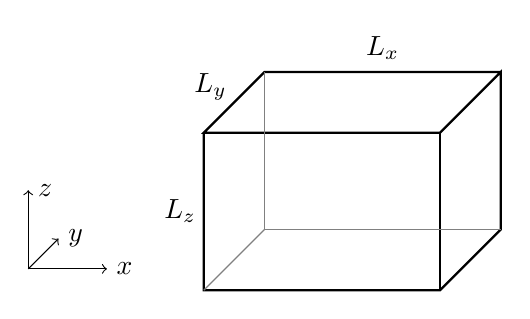
\begin{tikzpicture}
  \draw[thick](3,2,0)--(0,2,0)--(0,2,2)--(3,2,2)--(3,2,0)--(3,0,0)--(3,0,2)--(0,0,2)--(0,2,2);
  \draw[thick](3,2,2)--(3,0,2);
  \draw[gray](3,0,0)--(0,0,0)--(0,2,0);
  \draw[gray](0,0,0)--(0,0,2);
  \draw(1.5,2.3,0) node{$L_x$};
  \draw(-0.3, 2.2, 1) node{$L_y$};
  \draw(-0.3, 1, 2) node{$L_z$};
  
          %% Planes
        \coordinate (O) at (-3,-0.5,0);
        \coordinate (x) at (-2,-0.5,0);
        \coordinate (z) at (-3, 0.5,0);
        \coordinate (y) at (-3,-0.5,-1);
        \draw[->] (O) -- (x) node [right] {$x$};
        \draw[->] (O) -- (y) node [right] {$y$};
        \draw[->] (O) -- (z) node [right] {$z$};
\end{tikzpicture}
\caption{Imaginary box, fixed in space. You may think of this box being infinitesimally small.  We derive equations describing the mean quantities of the fluid in this box, as the fluid passes through this box. Eventually, we take the limits of $L_x$, $L_y$ and $L_z$ to zero, such that the box reduces to a single fixed point in space.}
\label{imaginary_box}
\end{center}
\end{figure}


In the equation above, the ``storage rate'' or ``tendency'' is the rate at which the amount of $X$ in the box is increasing.  The ``export rate'' or ``divergence'' is the rate at which $X$ is being carried by the fluid out of the box by passing through the walls of the box.  The ``sources'' are any addition of $X$ to the box (or, if negative, subtraction of $X$ from the box) through means other than being carried into or out of the box by the fluid flow.


To write out equation (\ref{conservation}) in more detail, note that the amount of $X$ in the box is equal to the volume of the box $V$ times the density of $X$.  So, the storage rate is\footnote{Here and throughout, the partial derivatives $\partial/\partial t$, $\partial/\partial x$, $\partial/\partial y$, and $\partial/\partial z$ will be abbreviated as $\ppt$, $\ppx$, $\ppy$, and $\ppz$.  This is simply a matter of convenience: it reduces clutter and saves ink.} $\ppt$ of the volume of the box $V$ times the density of $X$.  But, since $V$ is constant in time,
\[
\text{Storage rate of $X$ in the box} = V \ppt (\text{density of $X$}) \, .
\]
The export rate of $X$ is equal to the net rate at which $X$ is carried outwards across the faces of the box.  Let us consider the two faces whose normals are aligned with the $x$ axis. The rate at which $X$ passes through one of those faces is equal to the area of the face $L_y L_z$ times\footnote{Here, we adopt the standard meteorological convention of referring to the three components of the fluid velocity by $u$, $v$, and $w$, corresponding to $x$, $y$, and $z$ axes, respectively.} $u$ times the density of $X$.  The net sum across the two faces with $\hat{x}$ normals is then
\[
(L_y L_z) \left[ \left.(u \times\text{density of $X$})\right|_{+L_x/2} - \left.(u\times\text{density of $X$})\right|_{-L_x/2} \right] \, ,
\]
where the subscripts $-L_x/2$ and $+L_x/2$ indicate that the expressions should be evaluated at the location of these faces, which are at positions $-L_x/2$ and $+L_x/2$ relative to the box's center.  Now, if we imagine that our box is small compared to the spatial variations in $u$ or the density of $X$, then we can write\footnote{Mathematically, the expression must be divided by $L_x$ (or the volume $V=L_x L_y L_z$) before taking the limit of $L_x \rightarrow 0$, which is implicitly done when replacing the (small) finite difference in the $x$-direction by $\ppx$. For clarity, we keep $V$ for the moment, but will divide by it once we have collected expressions for all terms in the momentum equations.} this as
\begin{align}
& (L_y L_z) \left[ L_x \frac{\left.(u\times\text{density of $X$})\right|_{+L_x/2} - \left.(u\times\text{density of $X$})\right|_{-L_x/2}}{L_x} \right] \\
=& \; (L_y L_z) \left[ L_x \ppx (u\times\text{density of $X$}) \right] \\
=& \; V \ppx (u\times\text{density of $X$}) \, .
\end{align}
Similarly, the net amounts per time passing through the two $\hat{y}$-normal and $\hat{z}$-normal faces are
\[
V \ppy (v\times\text{density of $X$})
\]
and
\[
V \ppz (w\times\text{density of $X$}) \, .
\]
Altogether, the net amount of something being exported through the faces of the box is
\[
\text{Export rate of $X$ out of box} = V \grad \cdot \left(\vec{u} \times \text{density of $X$} \right) \, .
\]


The only thing left to figure out, then, are what the sources of $X$ are.  For mass, there are none:
\[
\text{Sources of mass to the box} = 0 \, .
\]
For momentum, there are gravity and pressure forces:
\[
\text{Sources of momentum to the box} = V \vec{g} - V \grad p \, .
\]
Here, $g = (0,0,-9.81\text{ m s$^{-2}$})$ is the gravitational acceleration vector and $p$ is the fluid pressure\footnote{Noting that the pressure of a fluid is isotropic (the same in all directions) and recalling that pressure is simply force per area, the pressure-gradient term $-V \grad p$ can be derived by considering the forces on the faces of the box.}.  For energy, radiation and pressure work are the sources of energy that we need to worry about\footnote{The diffusive flux of energy can be important, especially near the surface, but we will ignore that for simplicity.}:
\[
\text{Sources of energy to the box} = V Q - V \grad \cdot (p \vec{u})\, .
\]
Here, $Q$ is the net radiative heating per volume with units of W m$^{-3}$ and the last term represents the energy added to the box by being pushed by adjacent fluid at the faces of the box\footnote{Like the pressure-gradient term in the momentum equation, the $-V \grad \cdot (p \vec{u})$ term can be derived by .}.  Putting it all together, denoting the density of mass, momentum, and energy by $\rho$, $\rho\vec{u}$, and $\rho E$, and dividing by the constant $V$, we get
\begin{align}
\ppt \rho + \grad \cdot (\rho \vec{u}) &= 0 \label{mass_eulerian} \\
\ppt (\rho \vec{u}) + \grad \cdot (\rho \vec{u} \vec{u}) &= \rho \vec{g} - \grad p \label{momentum_eulerian} \\
\ppt (\rho E) + \grad \cdot (\rho E \vec{u}) &= Q - \grad \cdot (p \vec{u}) \, , \label{energy_eulerian}
\end{align}
where $E$ is the specific energy of the fluid\footnote{The term ``specific'' means ``per mass''.  Therefore, $E$ has units of J kg$^{-1}$.} and the pressure is specified by the ideal-gas law to be $p=R\rho T$, where $R$ is the specific gas constant of air.


\subsection{Energy $E = c_vT + u^2/2 + gz$}


What is $E$?  For a dry atmosphere, the energy in the box is a sum of three types: internal energy, kinetic energy, and gravitational potential energy.  Therefore, $E$ can be written as
\begin{equation}
E = \underbrace{c_v T}_{\text{internal}} + \underbrace{u^2/2}_{\text{kinetic}} + \underbrace{gz}_{\text{gravitational}} \, , \label{Edef}
\end{equation}
where $c_v \approx 700$ J kg$^{-1}$ K$^{-1}$ is the specific heat capacity of air at constant volume, $u$ is a shorthand\footnote{Note that $u$ is used for both the $x$ component of the wind and for the magnitude of the velocity.  This overloading of the variable $u$ is typical.  Context should make it clear which meaning is being used.} for $|\vec{u}| = \sqrt{u^2 + v^2 + w^2}$, and $g \approx 10$ m s$^{-2}$ is the magnitude of the gravitational acceleration.  Note that we made choices about what constitutes ``zero energy''.  For the internal energy, we have chosen ``zero internal energy'' to be at absolute zero.  For the kinetic energy, we have chosen ``zero kinetic energy'' to be when $\vec{u} = 0$ in our chosen reference frame.  For the gravitational potential energy, we have chosen ``zero gravitational potential energy'' to be at $z=0$ in our chosen reference frame.  We are always free to make these choices, or for that matter, any other set of choices.  To see why, note that we can multiply equation (\ref{mass_eulerian}) by any constant we want and add it to equation (\ref{energy_eulerian}); that effectively adds that constant to $E$, which can be interpreted as adding that constant to any one of the internal, kinetic, and gravitational energies, thereby changing where their zero-point values occur.


To understand the Earth's atmosphere, we must understand its energetics.  In particular, we need to understand how air parcels are able to move up and down in the atmosphere.  Moving laterally is pretty simple, but moving up and down requires an addition or removal of energy, either through phase changes of water or through radiative heating.  Since that up-and-down movement is utterly critical to how the atmosphere works, we need to understand its energetics.


Regarding the energetics, the simplest thing we can try to understand is the difference in energy between air at the bottom of the troposphere and air at the top of the troposphere.  Let us consider a static atmosphere; this lets us ignore the kinetic piece, whose contribution is small even in the real atmosphere\footnote{The highest winds in the atmosphere are about 40 m/s (80 mph), and that corresponds to a specific kinetic energy of $40^2/2 = 800$ J/kg, which is equal in energy to a temperature increment of about 1 K since $c_v = 700$ J kg$^{-1}$.  Therefore, we can safely ignore the kinetic piece in our order-of-magnitude energy calculations.}.  For our comparison, we will use nice, round numbers.  For the surface air, we will use $T = 300$ K and $z = 0$.  For air at the tropopause, we will use $T = 200$ K and $z = 15$ km.  At these two heights, we have:
\begin{align}
E \text{ @ surface} &= 700 \times 300 + 10 \times 0 \\
&= \num{210000} \text{ J kg}^{-1} \\
E \text{ @ tropopause} &= 700 \times 200 + 10 \times 15000 \\
&= \num{290000} \text{ J kg}^{-1} \\
\Delta E &= \num{290000} - \num{210000} = \num{80000} \text{ J kg}^{-1} \, .
\end{align}
Therefore, the tropopause air is {\text higher} in energy by \num{80000} J.


\begin{figure}
\begin{center}
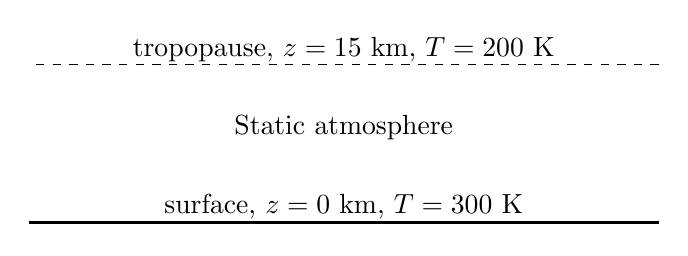
\begin{tikzpicture}
  \draw[dashed](8,0)--(0,0);
  \draw(4,0.2) node{tropopause, $z=15$ km, $T=200$ K};
  
  \draw[thick](8,-2)--(0,-2);
  \draw(4,-1.8) node{surface, $z=0$ km, $T=300$ K};
  \draw(4,-0.8) node{Static atmosphere};
\end{tikzpicture}
\end{center}
\caption{For the comparison of the energies of air at the surface and tropopause, we will assume that the tropopause is at 15 km and that the temperatures of the surface air and tropopause air are 300 and 200 K, respectively.}
\end{figure}


Is this the right way to calculate the energy difference?  The answer to that depends on what you are hoping to learn.  If we are interested in the movement of air up and down in the atmosphere, the answer is no: this difference in $E$ is {\it not} the energy that we must extract from a tropopause parcel by radiation to make it descend downwards to become a surface parcel.  Why?  There is the pressure term on the right-hand side of the governing equation for energy, $-\grad \cdot (p\vec{u})$, that prevents us from interpreting $\Delta E$ in this way.


\subsection{Internal energy $c_v T$}


What about internal energy?  Is it the ``right'' way to think about the energy difference between the lower and upper troposphere?  To find out, we need to derive the governing equation for internal energy.  This will not be a new equation; it can be derived from the equations we already have.


To get there, it will make things easier to first define the ``Lagrangian derivative'' $d/dt$, which is related to the Eulerian derivative $\partial/\partial t$ by
\begin{equation}
\ddt = \ppt + \vec{u} \cdot \grad \, . \label{ddt}
\end{equation}
The interpretation of the Lagrangian derivative is that it gives the rate of change following a parcel of fluid.  Contrast this with the Eulerian derivative, which gives the rate of change at a fixed point in space.


By the continuity equation, the momentum and energy equations can be written as
\begin{align}
\ppt \vec{u} + (\vec{u} \cdot \grad) \vec{u} &= \vec{g} - \frac{1}{\rho} \grad p \\
\rho \ppt E + \rho \vec{u} \cdot \grad E &= Q - \grad \cdot (p \vec{u}) \, .
\end{align}
By the definition of the Lagrangian derivative in equation (\ref{ddt}), this can be written as
\begin{align}
\frac{d}{dt} \vec{u} &= \vec{g} - \frac{1}{\rho} \grad p \\
\rho \frac{d}{dt} E &= Q - \grad \cdot (p \vec{u}) \, .
\end{align}
The former can be turned into a kinetic and potential energy equation by dotting with $\vec{u}$, 
\[
\frac{d}{dt} \left( \frac{1}{2} u^2 + gz \right) = - \frac{1}{\rho} \vec{u} \grad p \, .
\]
Multiplying by $\rho$ and subtracting from the $E$ equation gives
\begin{equation}
\rho \frac{d}{dt} (c_v T) = Q - p \grad \cdot \vec{u} \, . \label{internal}
\end{equation}


Let us compare the surface and tropopause.   At the surface, $T = 300$ K.  At the tropopause, $T = 200$ K.  Therefore,
\begin{align}
c_vT \text{ @ surface} &= 700 \times 300 \\
&= \num{210000} \text{ J kg}^{-1} \\
c_vT \text{ @ tropopause} &= 700 \times 200 \\
&= \num{140000} \text{ J kg}^{-1} \\
c_v \Delta T &= \num{140000} - \num{210000} = -\num{70000} \text{ J kg}^{-1} \, .
\end{align}
The tropopause air is {\it lower} in internal energy by \num{70000} J.


Does this difference in internal energy tell us about the energy that must be removed to bring a tropopause parcel down to the surface?  Certainly not.  If we believed that, then we would think that we have to heat a tropopause parcel to get it down to the surface.  This is not right.  The problem is in the remaining pressure term: $-p\grad\cdot \vec{u}$ (pdV work).


\subsection{Enthalpy $h = c_pT$}


Let us add $d(RT)/dt$ to both sides of equation (\ref{internal}).  On the left-hand side, this gives $d(c_p T)/dt$, where $c_p = c_v + R \approx 1000$ J kg$^{-1}$ is the specific heat capacity at constant pressure.  The right-hand side becomes
\begin{align}
& Q - p \grad \cdot \vec{u} + \rho \frac{d}{dt} (RT) \\
&= Q - p \grad \cdot \vec{u} + \frac{d}{dt}(\rho RT) - RT \frac{d}{dt} \rho \\
&= Q - p \grad \cdot \vec{u} + \frac{d}{dt} p + RT \rho \grad \cdot \vec{u} \\
&= Q - p \grad \cdot \vec{u} + \frac{d}{dt} p + p \grad \cdot \vec{u} \\
&= Q + \frac{d}{dt} p \, .
\end{align}
The result is the enthalpy equation,
\begin{equation}
\rho \frac{d}{dt} h = Q + \frac{d}{dt} p \, , \label{enthalpy}
\end{equation}
where $h = c_p T$ is the specific enthalpy for dry air.  Recall that ``specific'' means per mass.  What is enthalpy?  Enthalpy is the sum of internal energy plus $pV$.  Denoting the mass of fluid in the box by $M$, the specific $pV$ is $pV/M$, which equals $p/\rho$ since $M/V = \rho$, and $p/\rho = RT$ by the ideal-gas law ($p = R\rho T$).  Therefore, by adding $d(RT)/dt$ to both sides of the internal-energy equation, we changed our ``$X$'' from internal energy (which, per mass, is $c_v T$) to enthalpy (which, per mass, is $c_p T$).


Let us compare the surface and tropopause.   At the surface: $T = 300$ K, so $c_p T = 1000 \times 300 = 30 \times 10^4$ J/kg.  At the tropopause: $T = 200$ K, so $c_p T = 1000 \times 200 = 20 \times 10^4$ J/kg.  The tropopause air is lower in internal energy by 100,000 J.


Let us compare the surface and tropopause.   Again, the surface and tropopause temperatures are 300 and 200 K, respectively.  Therefore,
\begin{align}
c_pT \text{ @ surface} &= 1000 \times 300 \\
&= \num{300000} \text{ J kg}^{-1} \\
c_pT \text{ @ tropopause} &= 1000 \times 200 \\
&= \num{200000} \text{ J kg}^{-1} \\
c_p \Delta T &= \num{200000}-\num{300000} = -\num{100000} \text{ J kg}^{-1} \, .
\end{align}
The tropopause air is {\it lower} in internal energy by \num{100000} J.


This is still not the relevant thermodynamic variable for calculating the cooling needed to bring a parcel to the surface.  We still have a pesky pressure term on the right-hand side of equation (\ref{enthalpy}): $dp/dt$, which corresponds to the pressurization of the parcel.


\subsection{Potential temperature $\theta$}


To get rid of that pesky pressure term, let us divide both sides of equation (\ref{enthalpy}) by $\rho T$.  That produces
\[
c_p \ddt \log(T) = Q/(\rho T) + R \ddt \log(p) \, .
\]
This can be written as
\[
c_p \ddt \left[ \log(T) - \frac{R}{c_p} \log(p/p_0) \right] = \frac{Q}{\rho T} \, ,
\]
and then as
\[
\ddt \log(\theta) = \frac{Q}{c_p \rho T} \, ,
\]
or as 
\begin{equation}
\ddt \theta = \frac{\theta}{c_p \rho T} Q \, , \label{potential}
\end{equation}
where
\begin{equation}
\theta = T \left( \frac{p_0}{p} \right)^{R/c_p} \label{potdef}
\end{equation}
is called potential temperature.  The variable $\theta$ is the temperature that a parcel of air (with an initial pressure $p$ and temperature $T$) would have if adiabatically compressed or expanded to pressure $p_0$.  It is conventional to set $p_0 = 1 \text{ bar} = 10^5$ Pa, which approximates the surface pressure.  Note that we finally have an equation with no pressure terms on the right-hand side.  As we cool a parcel to bring it from the tropopause to the surface over time $\Delta t$, the change in its potential temperature is
\[
\Delta \theta = \frac{1}{c_p} \int_0^{\Delta t} dt \, \frac{\theta}{T} \frac{Q}{\rho} \, .
\]


Our ultimate goal is to find the specific cooling (J kg$^{-1}$) that is required to bring a tropopause air parcel down to the surface.  During the time $\Delta t$, the net specific cooling of the parcel is 
\[
\int_0^{\Delta t} dt \, \frac{Q}{\rho} \, .
\]
For the sake of intuition, it is sometimes convenient to talk about a heating or cooling in terms of Kelvins.  When we refer to ``$x$ K of heating'', we usually mean ``the Joules per kilogram of heating that would raise the temperature of an air parcel by $x$ K at constant pressure''.  These are simply related by a factor of $c_p$.  Specifically, we have the following correspondence:
\[
\int_0^{\Delta t} dt\, \frac{Q}{\rho} \quad [\text{J/kg}] \qquad \Longleftrightarrow \qquad \frac{1}{c_p} \int_0^{\Delta t} dt \, \frac{Q}{\rho} \quad [\text{K}] \, .
\]
Note that the right-hand side of (\ref{potential}) is not quite equal to this.  It has a factor of $\theta/T$ inside the integral.  Nevertheless, we can approximate that factor.
 

Let us compare the surface and tropopause.   At the surface, $T = 300$ K and $p = 10^5$ Pa, so $\theta = 300 (1)^{R/c_p} = 300$ K.  At the tropopause, $T = 200$ K and $p = 0.13 \times 10^5$ Pa, so $\theta = 200 (1/0.13)^{R/c_p} = 360$ K.  We do not know the time-averaged $\theta/T$, but we can approximate $\theta$ and $T$ in that ratio as averages of their tropopause and surface values, which are $(360+300)/2 = 330$ K and $(200+300)/2 = 250$ K, respectively.  Then,
\begin{align}
\Delta \theta &= \frac{1}{c_p} \int_0^{\Delta t} dt \, \frac{\theta}{T} \frac{Q}{\rho} \\
&\approx \frac{1}{c_p} \frac{330}{250} \int_0^{\Delta t} dt \, \frac{Q}{\rho} \\
\Rightarrow \quad \frac{1}{c_p} \frac{330}{250} \int_0^{\Delta t} dt \, \frac{Q}{\rho} &\approx \frac{250}{330} (360-300) \\
&\approx 45 \text{ K} \, .
\end{align}
This is roughly the amount of cooling needed to bring a tropopause parcel down to the surface.


\subsection{Entropy $c_p \log \theta$}


It is worth noting at this stage that $c_p \log \theta$ is the entropy of dry air.  We can derive its governing equation from (\ref{potential}), which gives
\[
\ddt \left( c_p \log \theta \right) = \frac{Q}{\rho T} \, .
\]
Note the familiar ``heating divided by temperature'' term on the right-hand side.  And, note this equation does not contribute any new information not already present in our governing equations for mass, momentum, and energy; in fact, we have derived this equation purely from the conservation of mass, momentum, and energy.


\subsection{Dry static energy $\text{DSE} = c_p T + gz$} \label{subsec_dse}


Potential temperature is nice because it is so well conserved, but with its exponents and its source that is not exactly equal to specific heating, it is inconvenient.  A more convenient equation can be obtained from the enthalpy equation so long as we do not mind invoking hydrostatic balance.  Assuming that the atmosphere is hydrostatic and that we cool or heat parcels slowly enough that they are always at their equilibrium height (i.e., their density equal to the environment's density), then
\begin{align}
\frac{d}{dt} p &= \ppt p + \vec{u} \cdot \grad p \\
&= w \ppz p \\
&= -w\rho g \\
&= -\rho \frac{d}{dt} (gz) \, .
\end{align}
Using this to rewrite the $dp/dt$ term in equation (\ref{enthalpy}), the enthalpy equation becomes
\[
\rho \frac{d}{dt} (c_p T) = Q - \rho \frac{d}{dt} (gz) \, ,
\]
or
\begin{equation}
\frac{d}{dt} \dse = Q/\rho \, , \label{dse}
\end{equation}
where $\dse{} = c_p T + gz$ is the dry static energy.  Now, we have a very clean relationship between a function of the parcel's state (DSE) and the specific heating ($Q/\rho$).


Let us compare the surface and tropopause.   At the surface, $T = 300$ K and $z = 0$.  At the tropopause, $T = 200$ K and $z = 15$ km.  Therefore,
\begin{align}
\dse \text{ @ surface} &= 1000 \times 300 + 10 \times 0 \\
&= \num{300000} \text{ J kg}^{-1} \\
\dse \text{ @ tropopause} &= 1000 \times 200 + 10 \times 15000\\
&= \num{350000} \text{ J kg}^{-1} \\
\Delta \dse &= \num{350000}-\num{300000} = \num{50000} \text{ J kg}^{-1} \, .
\end{align}
The tropopause air is {\it higher} in dry static energy by 50,000 J kg$^{-1}$.  Dividing by $c_p = 1000$ J kg$^{-1}$ K$^{-1}$, this corresponds to 50 K.  So, we see that our approximate calculation of 45 K from the $\theta$ equation was pretty close to the actual answer.


Needless to say, DSE is super useful.  It has gotten us the amount of cooling needed to bring a parcel from the tropopause to the surface, or, vice versa, the amount of heating to bring a parcel from the surface to the tropopause.  In the absence of heating, DSE is conserved (so long as we obey the conditions).  So, if we lift a parcel from the surface to the tropopause without any heating, then its original DSE of $30 \times 10^4$ J/kg is conserved, so the temperature becomes $(30 \times 10^4 - 10 \times 15000)/1000 = 150$ K.  Not surprisingly, that is 50 K less than the temperature of the tropopause air; this is the 50 K that must be added as we lift the parcel if we want it to be neutrally buoyant at the tropopause.


Note that we can restate all of this very simply.  Conservation of DSE implies that $dT/dz = -g/c_p = -10$ K/km.  This is just the dry adiabatic lapse rate.  As atmospheric scientists, we recite this ten times before we go to bed and ten times when we wake up.


But, do not use conservation of DSE blindly.  If we lift the surface parcel to 40 km in the stratosphere, what will the temperature of the parcel be?  As we saw above, a parcel with a temperature of 300 K at the surface has a DSE of 300 kJ kg$^{-1}$.  

At 40 km, the parcel's DSE would be
\[
\dse{} = 1000 T + 10 \times 40000 \, ,
\]
where $T$ is the unknown temperature of the parcel there.  To solve for $T$, we use conservation of DSE, which tell us that this expression is equal to 300 kJ kg$^{-1}$.  Therefore,
\begin{align}
1000 T + 400000 &= 300000 \\
\Rightarrow \quad 1000 T &= -100000 \\
\Rightarrow \quad T &= -100 \text{ K} \, .
\end{align}
Negative temperature!  What went wrong?  Can we not lift a parcel to 40 km?  Of course we can.  That is a totally physical thing to do.  And, since negative temperatures are meaningless, it is conservation of DSE that must have failed.  We will find out why later.


\section{Tropospheric energy balance}


Clear air cools by radiative cooling (primarily infrared emission) by about 1 K per day.  Since there are 10 tons ($10^4$ kg) of air overlying each square meter of surface, and about $10^5$ seconds in a day, that corresponds to about
\[
M c_p \left( \frac{1}{c_p} \frac{Q}{\rho} \right) = 10^4 \times 1000 \times 10^{-5} = 100 \text{ W m$^{-2}$} \, .
\]
That is a lot of cooling.  How is this balanced?  By the definition of the Lagrangian derivative in equation (\ref{ddt}),
\[
\ddt \dse = \ppt \dse + u \ppx \dse + v \ppy \dse + w \ppz \dse \, .
\]
In the tropics, $\ppt T$ is nearly zero, as are $\ppx T$ and $\ppy T$.  Therefore, equation (\ref{dse}) can be approximated as
\[
w \ppz \dse \approx Q/\rho \, .
\]
In other words, radiative cooling of clear air is balanced by descent of the clear air (vertical advection of higher $\dse{}$ from aloft).  This is illustrated in Figure \ref{17leshouches_descent_dse}.  We can draw the same diagram in terms of $T$.  This is shown in Figure \ref{17leshouches_descent_tabs}.


\begin{figure}
\begin{center}
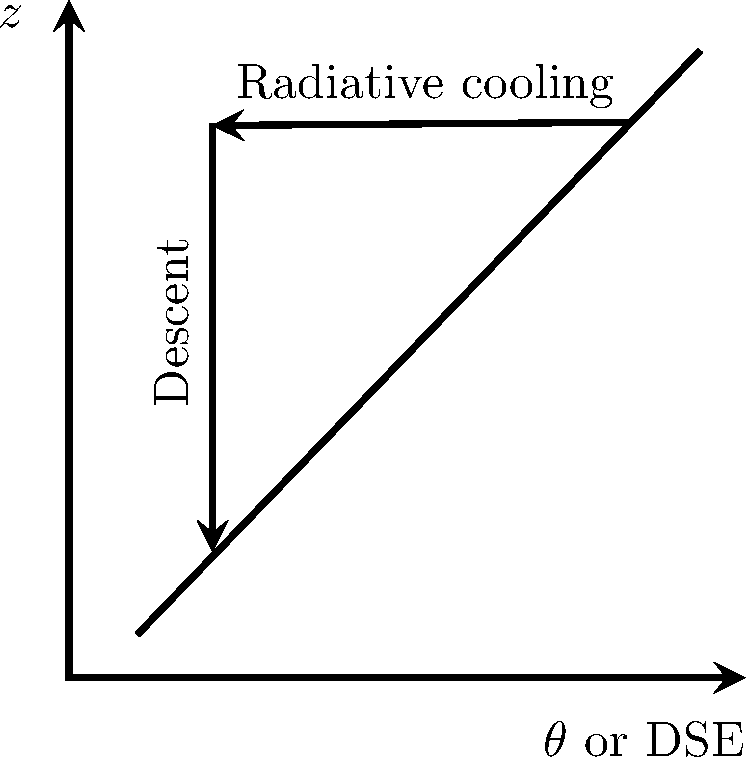
\includegraphics[width=3in]{../figures/17leshouches_descent_dse.pdf}
\caption{A schematic of the clear-sky thermodynamic balance from the perspective of $\theta$ or DSE.  Clear-sky radiative cooling moves the parcel to the left in this diagram.  Since $\theta$ and DSE are conserved for adiabatic processes, descent of the parcel moves the parcel downward in this diagram.  In a steady state, Lagrangian parcels move, but they move along the existing thermodynamic profile, which keeps the profile constant in time.}
\label{17leshouches_descent_dse}
\end{center}
\end{figure}


\begin{figure}
\begin{center}
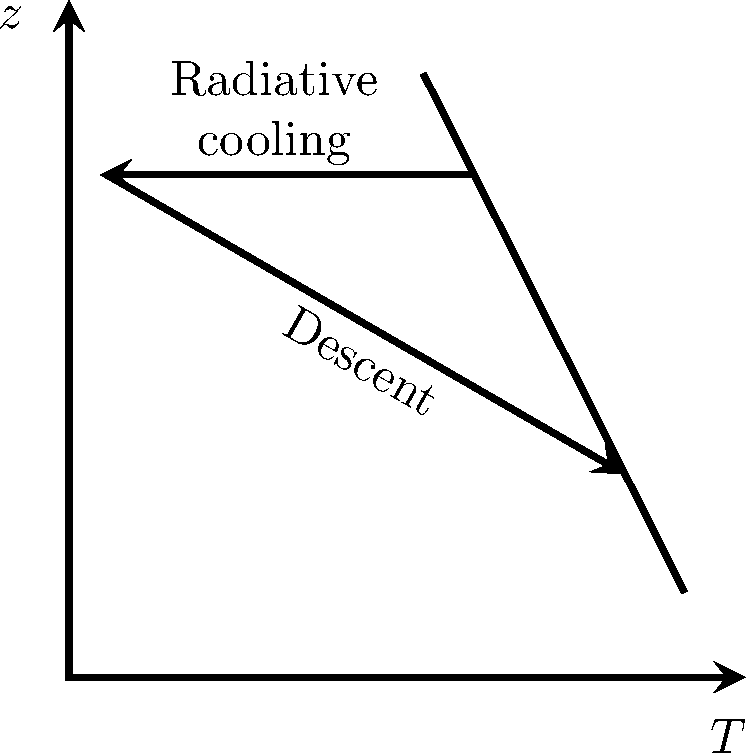
\includegraphics[width=3in]{../figures/17leshouches_descent_tabs.pdf}
\caption{A schematic of the clear-sky thermodynamic balance from the perspective of $T$.  Clear-sky radiative cooling moves the parcel to the left in this diagram.  Since an adiabatically descending parcel has a dry-adiabatic lapse rate $g/c_p = 10$ K/km that is larger than $-ppz T$, descent of the parel moves the parcel down and to the right in this diagram.  In a steady state, Lagrangian parcels move, but they move along the existing temperature profile, which keeps the profile constant in time.}
\label{17leshouches_descent_tabs}
\end{center}
\end{figure}


Note that the clear air is everywhere sinking.  What makes that possible?  Where does that air come from?  Why is there a seemingly endless source of air at high altitudes?  The answer is that the high-altitude air is supplied by clouds!  Clouds are the only thing that can power their way up through the atmosphere to dump air at high altitudes.  Those cloudy convecting parcels move so quickly that radiation does not have time to act.  Instead, the balance is between vertical advection and latent heating.  Denoting clear air by a subscript $e$ for environment and denoting convection by a subscript $c$, we can think of this as
\[
w_c \ppz \dse = Q_{c,\text{condensation}} / \rho \, ,
\]
where the subscript $c$ reminds us that this equation is meant for within clouds.  Now, some of the condensates that form within the cloud end up evaporating in the environment, either because cloudy air detrains into the environment and evaporates or because rain falls through the environment and evaporates.  This produces an additional cooling of the environment, so we should write the environmental DSE balance as
\[
w_e \ppz \dse{} = \Big[ Q_{e,\text{radiation}} + Q_{e,\text{evaporation}} \Big] / \rho \, ,
\]
where the subscript $e$ reminds us that this equation is meant for the environment.


The atmosphere's energy cycle works like this: the Sun heats the ocean, the ocean cools itself by evaporating water, the resulting water vapor is used by clouds to power their way to the upper troposphere, that causes subsidence everywhere else by continuity, and that adiabatic heating by subsidence is matched by radiative and evaporative cooling.  Sounds simple enough, but there are a lot of questions:
\begin{itemize}
\item What sets the value of $\ppz \dse{}$ or, equivalently, $T(z)$? 
\item What sets $Q_{e,\text{radiation}}$ or, equivalently, what sets the distribution of humidity?
\item What sets $Q_{e,\text{evaporation}}$ or, equivalently, what is the fate of condensed water?
\item How is $Q_{c,\text{condensation}}$ affected by the turbulent entrainment of dry air?
\end{itemize}
These are some of the biggest unresolved questions in atmospheric science.


\section{How do GCMs work?}


In Earth's atmosphere, cloudy updrafts have a typical width of around 1 km.  Global climate models (GCMs), on the other hand, have a typical grid spacing that ranges from 25--200 km.  Therefore, the GCM grid spacing is much too large to resolve cloudy updrafts, at least not motions that faithfully represent true moist convection.  


To understand how GCMs deal with this problem, it is sufficient to consider a single column of a GCM.  In fact, a single column of a GCM is often isolated and used for research purposes all on its own.  Isolated in this way, we call such a thing a single-column model (SCM).  But how can an SCM possibly capture the dominant energy balance in the clear air?  As we have learned, the radiative cooling of clear air is balanced by having the clear air sink.  In an SCM, however, there is nowhither for the air to go, and nowhence to come.


Since the cloudy updrafts cannot be resolved explicitly, their effects must be parameterized.  Fortunately, in addition to being small, cloudy updrafts also occupy a small fraction of area: a typical fraction of area that is occupied by cloudy updrafts is on the order of $10^{-3}$--$10^{-2}$.  As a consequence, there are two conceptual frameworks that we could use for parameterizing cloudy updrafts in an SCM.  Both take advantage of the fact that cloudy updrafts occupy a very small area.


In the first framework, we let the GCM grid column represent just the clear air, and let convection be an appropriate source or sink of air at each height.  This is depicted in Figure \ref{17leshouches_scm}a, in which a blue tube represents cloudy air being removed from the lower part of the clear-air-only grid column and deposited into the upper part of the column.  Let us define the mass flux of cloudy air $M$ as the kilograms of air per second that go up the tube divided by the horizontal area of the grid column.  By mass continuity, the vertical velocity $w$ of the air in the grid column in between the tube's inlet and outlet must be given by
\begin{equation}
w = - M/\rho \, . \label{framework1_mass}
\end{equation}
In a steady state, this subsidence must be balanced energetically by radiative and evaporative cooling.  Therefore, the vertical velocity of the column is related to those processes by
\begin{equation}
w \ppz \dse = \left( Q_{\text{radiation}} + Q_{\text{evaporation}} \right) / \rho \, . \label{framework1_energy}
\end{equation}
Do not be confused by the fact that there are two equations here for $w$.  The way to think about this is that the cooling from $Q_{\text{radiation}} + Q_{\text{evaporation}}$ sets $w$ by energy conservation, and then $w$ sets $M$ by mass conservation.  In this first scenario, note that the convection must be parameterized in two places: the $M$ in the mass equation and the $Q_{\text{evaporation}}$ in the energy equation.  (In practice, convection must also be parameterized in the momentum and humidity equations, but we are ignoring those for simplicity.)


\begin{figure}
\begin{center}
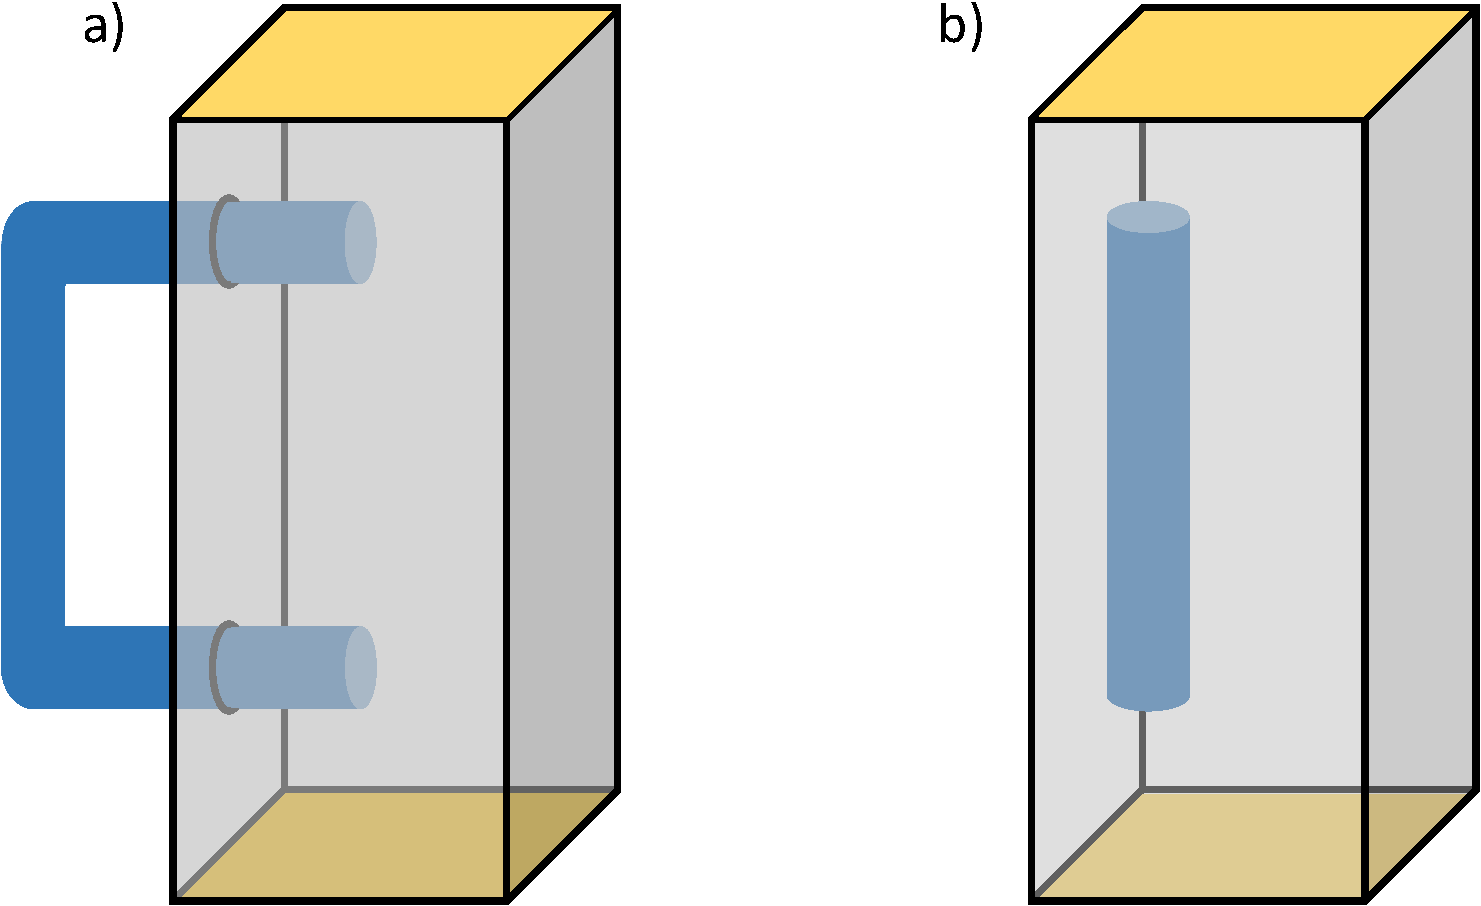
\includegraphics[width=3in]{../figures/17leshouches_scm.pdf}
\caption{Two possible frameworks for incorporating moist convection into a GCM grid column.  (a) In the first framework, we think of all of the air in the grid column as being clear environmental air, and we imagine that the convection is a sink and source of mass throughout the column, which we can visualize as cloudy air moving upward through tubes outside the grid column.  (b) In the second framework, we think of the air in the grid column as including both the clear environmental air and moist convection, so the tube carrying cloud updrafts lies within the grid column.  This second framework is the one used in most, if not all, GCMs.}
\label{17leshouches_scm}
\end{center}
\end{figure}


In the second framework, we let the GCM grid column represent an average over all the air: cloudy updrafts and clear air.  This is depicted in Figure \ref{17leshouches_scm}b, in which a blue tube representing the cloudy updrafts is within the grid column.  In this second framework, the vertical velocity $w$, which now represents an average of cloudy and clear, must be zero in a steady state: there can be no net vertical movement of mass in a steady-state closed box.  Therefore,
\begin{equation}
w = 0 \, . \label{framework2_mass}
\end{equation}
If $w = 0$, how is energy conservation satisfied?  Even though there is no net vertical movement of mass, 99--99.9\% of the air in the grid column is descending at levels between the tube's inlet and outlet.  This is because the tube itself (the cloudy updrafts) occupy only 0.1--1\% of the horizontal area.  So, the mass flux in the tube is still causing the the vast majority of the column to sink even though it does not register in the column's $w$.  The energy balance is now
\begin{equation}
0 = Q_{\text{radiation}} + Q_{\text{evaporation}} + Q_{\text{subsidence}} \, , \label{framework2_energy}
\end{equation}
where
\[
Q_{\text{subsidence}} = -M \ppz \dse{} \, .
\]
Since the vertical velocity of the clear environment is $w_e = -M/\rho$ by mass conservation, this is basically the same as equation (\ref{framework1_energy}), but written with the subsidence term on the right-hand side.  In this second framework, the convection must be parameterized in only one place: the sum of $Q_{\text{evaporation}} + Q_{\text{subsidence}}$, which is the convective tendency for dry static energy.


To the best of the author's knowledge, all GCMs are written with the second framework in mind, depicted in Figure \ref{17leshouches_scm}b.  This has the advantage of not treating the cloudy updrafts as contained within the grid column, but it has the disadvantage of hiding a lot of advection.  In an SCM, stuff in the column (water vapor, trace gases, momentum) must be advected downward by the convective parameterization.  And advection is one of the hardest things to do well in any numerical simulation of fluids.  So, it is important to be aware that the dynamical core (dycore, for short) is not the only piece of a GCM responsible for the challenging numerical task of advecting fluid.


With either approach, the balance that is achieved in this single column is referred to as radiative-convective equilibrium (RCE).  As its name implies, this is a steady state in which radiative cooling is balanced with convective heating.  Typically, this refers to solutions in which there is no net ascent in the column (i.e., for approach 2, $w = 0$).  RCE is an excellent starting point for understanding the structure of the tropical atmosphere.


\section{Rigid-lid gravity waves}


In a GCM, each column has neighbors so it is no longer ``single''.  And, since a grid column can import and export mass through its lateral boundaries, its $w$ is no longer required to be zero even in a steady state.  If there is a lot of cloudy mass flux in the column, then $w$ will be positive, indicating that the column is ascending on average.  If there is very little cloudy mass flux, then $w$ will be negative (due to the fact that the environmental air is subsiding to balance the radiative cooling).  To first approximation, we can think of the clear air as descending at the same speed everywhere in the free troposphere, so it is the variation in cloud ascent that causes a column's $w$ to have one sign or the other.


What kind of flow through the lateral boundaries of a grid column allow it to ascend or descend?  Consider a two-dimensional atmosphere ($x$ and $z$) that is split up into adjacent columns.  Imagine that, initially, $w$ is zero in each column; in other words, the upward cloudy mass flux in each column is exactly balanced by the downward flux of environmental air.  Then, imagine that one of the column briefly has more moist convection than normal.  What happens?  By mass conservation, the environmental air in that column must briefly descend ore than normal.  That puts the subsidence out of balance with the radiative cooling, causing the column to heat up.  Now, the column is warmer than its surroundings.  Recall that the clear environmental air occupies 99-99.9\% of the column, so this means that the environmental air is warmer than the environmental air in the surrounding columns.  Since warm air rises, a circulation develops between the column and its nearest neighbors, allowing the column to have $w > 0$ through a brief ascent (or a brief decrease in the descent rate) of the environmental air.  Of course, by mass conservation, this means that the neighboring columns must descend, i.e., have $w < 0$.  So, their environmental air warms up a bit.  They now want to ascend, and they do, but that causes {\it their} neighbors to descend, and so on.  This is a gravity wave.


Describing gravity waves in a compressible atmosphere with a realistic stratification is a pain in the neck.  Fortunately, we can work with a simplified system to get some physical intuition for these waves.  The simplest system with gravity waves is the 2D shallow-water system.  But, such a system does not allow us to think about vertical structure and vertical propagation of waves.  For that, we need to work with a Boussinesq fluid.


The Boussinesq equations describing hydrostatic linear perturbations to a two-dimensional, nonrotating, stratified fluid at rest are
\begin{subequations}\label{2dbouss_eqns}
\begin{eqnarray}
\partial_t u &=& -\frac{\partial_x p}{\rho_0}  \label{hmom}  \\
0 &=& -\frac{\partial_z p}{\rho_0} + b  \label{vmom}  \\
\partial_t b &=& -N^2 w + Q \label{therm}  \\
0 &=& \partial_x u + \partial_z w \, , \label{cont}
\end{eqnarray}
\end{subequations}
where $u$ is the horizontal speed, $w$ is the vertical speed, $\rho_0$ is a constant density, $p$ is the pressure perturbation, $b$ is the buoyancy, $N$ is the Brunt-V\"ais\"al\"a frequency, and $Q$ is the buoyancy source or, in other words, the heating.  Let there be a rigid lid at $H$, where $H$ is the tropopause.


With this system of equations, we will want to understand what happens when we have an isolated pulse of heating.  This isolated pulse of heating can be thought of as either the subsidence warming generated in the vicinity of a single cumulonimbus, or as the heating of a column of atmosphere due to a positive anomaly in the convective mass flux in that column.  Either way, if we imagine the vicinity of the cumulonimbus is small (or that the column that got anomalously heated is small), then we can approximate that heating as being localized as a Dirac delta function in $x$.  Likewise, if the heating is deposited quickly, then we can think of the heating as being localized in time.  On the other hand, the vertical structure of the heating could be anything.  To simplify matters, we use sine functions to describe different possible vertical structures.  (These sine functions can be used to construct any vertical structure of heating that is zero at the surface and tropopause.)  Let $m$ be the vertical wavenumber of the chosen sine function: $m = n\pi/H$, where $n$ is an integer.  Then, a heating that is localized in $x$, localized in $t$, and has vertical wavenumber $m$ is described mathematically by
\begin{equation}
Q(x,z,t) = B_0 \sin(mz) \mathcal{H}(H-z) \delta(x) \delta(t) \, . \label{bsource}
\end{equation}
Here, $B_0$ is the horizontally integrated amplitude of the resulting buoyancy anomaly at $t=0^+$.  In fact, equation (\ref{therm}) tells us that the buoyancy at time $t=0^+$ is simply
\begin{equation}
b_m(x,z,0^+) = B_0 \sin(mz) \mathcal{H}(H-z) \delta(x) \, , \label{b_initial}
\end{equation}
where we will keep a subscript $m$ on this buoyancy to remind us that this is the solution with that vertical wavenumber.  The question, then, is how this buoyancy evolves in time.  In other words, what is $b(x,z,t)$ for $t>0$?


To begin, we must first obtain from equations (\ref{2dbouss_eqns}) a single equation for $b$.  The reader can verify that we obtain
\begin{equation}
\partial_t^2 \partial_z^2 b + N^2 \partial_x^2 b = \partial_t \partial_z^2 Q \, , \label{b_wave}
\end{equation}
Since we already know the buoyancy at $t=0^+$, and since $Q=0$ for all $t>0$, we are interested in the homogeneous part of this equation, i.e.,
\begin{equation}
\partial_t^2 \partial_z^2 b + N^2 \partial_x^2 b = 0 \, . \label{b_wave_homo}
\end{equation}
This looks an awful lot like a wave equation.


To make any further progress, though, we need to make an assumption about the boundary condition at the tropopause.  It is typical to treat the tropopause as a rigid lid.  This is tantamount to assuming that the static stability of the stratosphere is infinite; i.e., $N = N_1 > 0$ in the troposphere, where $N_1$ is finite, and $N = N_2 = \infty$ in the stratosphere.  That infinite stratification implies that $w = 0$ at the $z = H$.  Since $w$ also equals zero at the surface, i.e., at $z=0$, we have a finite domain in the vertical, and this implies that the normal modes of the system are discretized.  In fact, from looking at equation (\ref{b_wave_homo}), we can guess them pretty easily:
\[
\sin(mz) f(x + Nt/m)
\]
and
\[
\sin(mz) f(x - Nt/m) \, ,
\]
with $m$ an integer multiple of $\pi/H$ and $f$ an arbitrary function.


So, the solutions are waves of buoyancy that retain their vertical structure and propagate either to the left or the right with speed $N/m$.  Therefore, for the initial buoyancy given in equation (\ref{b_initial}), the solution must be a delta function moving either to the left and/or the right.  In fact, by the symmetry of the problem, there must be equal delta functions moving to the left and the right.  Therefore, the solution is
\begin{equation}
b_m(x,z,t) = \frac{B_0}{2} \Big[ \delta(N_1 t/m + x) + \delta(N_1 t/m - x) \Big] \sin(m z) \mathcal{H}(H-z)\mathcal{H}(t)  \, . \label{b_rigid}
\end{equation}
In the absence of dissipation, these pulses will propagate forever.  As more and more moist convection happens, the domain fills up with more and more of these pulses, adding more and more kinetic energy.  When does the growth in kinetic energy ever stop?  In this system, never.


\section{Leaky-lid gravity waves}


In the real atmosphere, this does not happen.  Why?  Because the tropopause is not a rigid lid.  The stratification of the stratosphere is not infinite.  Instead, $N_2$ is positive and finite.  In this case, we now have a semi-infinite atmosphere in the vertical, and $N$ is piecewise constant in height such that
\begin{eqnarray}
N = \begin{cases}
N_1 & 0 \le z \le H \\
N_2 &  H < z
\end{cases} \, .
\end{eqnarray}
When $N_2 > N_1$, this is a simple analogue for Earth's atmosphere in which the troposphere is capped by the more stratified stratosphere.


Now, we have to be a bit more careful when we describe the heating.  In principle, we could add a heating to the stratosphere.  In practice, moist convection does not get up there, so we are still only interested in heatings that are confined between $z=0$ and $z=H$.  Therefore, we just need to be clear that our wavenumber-$m$ heating pulse and the resulting initial buoyancy is restricted to $z<H$, which we can do with the Heaviside unit step function $\mathcal{H}$,
\begin{equation}
b_m(x,z,0^+) = B_0 \sin(mz) \delta(x) \mathcal{H}(H-z) \, . \label{b_initial_leaky}
\end{equation}
How does this evolve in time?  Is (\ref{b_rigid}) the solution?  No, it is not.  Since there is no longer a rigid lid, $w$ is no longer constrained to be zero there, and the normal modes are now quite different.  However, $b_m(x,z,t)$ can be derived analytically; for details, see \citet{15leaky}.


Although the expression for $b_m(x,z,t)$ is a bit complicated, its behavior is simple.  There are still two pulses of buoyancy: one that travels left and one that travels right.  And, as in the rigid-lid case, the pulses are initially delta functions and they travel away from the origin at a speed of $N/m$.  But, there are two big differences from the rigid-lid case: the stratosphere jiggles with waves, and the pulses in the stratosphere melt.  In particular, each pulses grows in width linearly with time.  As a function of time, the full-width half-maximum of each pulse is
\[
\text{FWHM} \approx \frac{N_1}{N_2} \frac{\pi N_1 t}{H m^2} \, .
\]
Since the integrated buoyancy within each pulse is finite, this also means that the buoyancy in each pulse is finite valued for all $t>0$.


Let us put some numbers to these things.  For $N_1 = 0.01$ s$^{-1}$, $N_2 = 0.025$ s$^{-1}$, $m = \pi/H$, and $H = 15$ km (characteristic values for Earth's tropics), 
\begin{align}
d\text{FWHM}/dt &\approx \frac{N_1}{N_2} \frac{H N_1}{\pi} \\
&\approx \frac{.01}{.025} \frac{15 \times 10^3 \times .01}{3} \\
&= 20 \text{ m/s} \, .
\end{align}
Meanwhile, for a first-baroclinic wave ($m = \pi/H$), the horizontal group velocity is
\begin{align}
c_{gx} &= N_1/m \\
&= \frac{H N_1}{\pi} \\
&\approx \frac{15 \times 10^3 \times 0.01}{3} \\
&= 50 \text{ m/s} \, .
\end{align}
So, we see that the speed which which each pulse widens is comparable in magnitude to its speed of propagation.


How can we understand this behavior?  Putting a plane wave $b_m \propto \exp(-i\omega t + ikx + imz)$ into 
\[
\partial_t^2 \partial_z^2 b_m + N^2 \partial_x^2 b_m = 0 \, ,
\]
we find
\[
(i\omega)^2 (im^2)+ N^2 (ik)^2 = 0 \, ,
\]
which can be written as
\[
\omega = \pm N k/m \, .
\]
This is the dispersion relation for hydrostatic gravity waves in the troposphere.  The vertical group velocity is
\[
c_{gz} = \frac{\partial \omega}{\partial m} = \mp N_1 k/m^2 \, .
\]
Taking the plus sign so that the wave packets travel upwards, we get $N_1k/m^2$.  To get an estimate of the residence time of the wave energy in the troposphere, we divide $H$ by this speed and get
\[
\tau_{\text{no lid}} \approx \frac{m^2 H}{N_1 k} \, .
\]
This is the timescale with no lid, i.e., with $N_2 = N_1$.  When $N_2 > N_1$, there is some wave reflection at the tropopause, trapping wave energy for longer.  The result is that residence timescale is increased by a factor of $N_2/N_1$; see \citet{15leaky} for details.  Therefore, the residence timescale for a wave with wavenumbers $k$ and $m$ is
\[
\tau_{\text{leaky lid}} \approx \frac{N_2}{N_1} \frac{m^2 H}{N_1 k} \, .
\]
In the tropics, $N_2/N_1 \approx 2.5$ and $H \approx 15$ km.  The key thing for us to note is tha this timescale is proportional to $1/k$, so higher horizontal wavenumbers decay faster.  A wave with a first-baroclinic ($m = \pi/H$) vertical structure and a 100-km horizontal wavelength will decay on a timescale of
\begin{align}
\tau_{\text{leaky lid}} &\approx \frac{N_2}{N_1} \frac{m^2 H}{N_1 k} \\
&= 2.5 \frac{\pi^2}{15 \times 10^3 \times 0.01 \times (2\pi/10^5)} \\
&= 2.5 \frac{\pi}{3 \times 10^{-3}} \\
&\approx 2500 \text{ s} \\
&\approx 40 \text{ minutes} \, .
\end{align}
After an hour, what is left?  That depends on what we started with.  If we only had that one component, i.e., a first-baroclinic vertical structure with buoyancy alternating between positive and negative sinusoidally with a wavelength of 100 km, then not much: that pattern has mostly disappeared by 1 hour.  If the pattern were not sinusoidal, but still had a wavelength of 100 km, then there would have been higher-$k$ components at the beginning, but those would have decayed away even faster than 1 hour because the residence timescales goes like $1/k$.  On the other hand, if there were components with wavelengths greater than 100 km, then they would still remain.


The longest-lived first-baroclinic wave would be the wave with the longest possible horizontal wavelength.  On Earth, the maximum lengthscale is set by the planet's circumference of 40,000 km.  For a wave with that horizontal wavelength, the timescale would be 400 times as long as for the 100-km wavelength, and that is equal to about 10 days.


It is important to recognize that the vertically propagating waves do {\it not} remove the horizontally averaged buoyancy from the troposphere.  The horizontally averaged buoyancy belongs to the $k=0$ component, which has an infinite residence timescale.  The propagation of waves out of the troposphere simply smooths the buoyancy horizontally until, finally, it is horizontally uniform.


\section{When and why does DSE conservation fail?}


In section \ref{subsec_dse}, we saw that using conservation DSE could generate negative temperatures, which is clearly unphysical.  The problem is that the standard DSE equation, which we had written (and is almost always written) as
\[
\frac{d}{dt} \dse = Q/\rho \, ,
\]
is actually wrong.  To find out what went wrong, and to correct it, we must go back to the enthalpy equation,
\[
\rho \frac{d}{dt} h = Q + \frac{d}{dt} p \, .
\]
To treat the $dp/dt$ term properly, we need to distinguish between the pressure and density of the Lagrangian parcel ($p$ and $\rho$) and the pressure and density of the environment far from the Lagrangian parcel ($p_e$ and $\rho_e$).  Then, to invoke hydrostatic balance, we need to make two reasonable assumptions: 1.~that the environment is hydrostatic far from the parcel (with $\ppz p_e = -\rho_e g$ there) and, 2.~that $p(z) = p_e(z)$ (which does {\it not} require hydrostatic flows around the parcel).  With those two assumptions,
\begin{align}
\frac{dp}{dt} &= \frac{dp_e}{dt} \\
&= w \frac{dp_e}{dz} \\
&= w \ppz p_e \\
&= -w \rho_e g \\
&= -\rho_e \ddt (gz) \, .
\end{align}
Substituting into the enthalpy equation, we get
\[
\rho \ddt h = Q - \rho_e \ddt (gz) \, .
\]
Next, we add $\rho d(gz)/dt$ to both sides to make $\rho d\dse{}/dt$ on the left.  Because $\rho_e \neq \rho$ in general, we get
\[
\rho \ddt \dse{} = Q + (\rho - \rho_e) \ddt (gz) \, .
\]
Dividing by $\rho$, this can be written as
\begin{equation}
\ddt \dse{} = Q/\rho - b w \, , \label{dse_corrected}
\end{equation}
where
\begin{equation}
b = g (1 - \rho_e/\rho)
\end{equation}
is the parcel's buoyancy.  For adiabatic processes,
\[
\ddz \dse{} = -b \, .
\]
In other words, if the Lagrangian parcel is positively buoyant, then its DSE decreases with height.  If it is negatively buoyant, its DSE increases with height.  We can write this as a conservation law by noting that convective available potential energy (CAPE) is the vertical integral of a parcel's buoyancy from its current height to some reference height above (e.g., its level of neutral buoyancy),
\[
\text{CAPE} = \int_z^{\text{LNB}} dz' b(z') \, .
\]
Note that
\[
\frac{d}{dz} \text{CAPE} = -b \, .
\]
Therefore, we can write the general conservation law for a dry adiabatically lifted parcel as
\[
\frac{d}{dz} \left( \text{DSE} - \text{CAPE} \right) = 0 \, .
\]
In other words, $\dse{}-\text{CAPE}$ is conserved for an adiabatically lifted parcel.  When water is involved, the correct statement is that {\it moist} static energy (MSE) minus CAPE is conserved; see \citet{15mse} for details.


Let us return to that example of lifting a surface parcel to 40 km.  Using an original temperature of 300 K and conserving DSE, we got the nonsensical temperature of $-100$ K.  Now, let us use conservation of $\dse{}-\text{CAPE}$.  That can be written as
\begin{align}
\ddz \left( c_p T + gz \right) &= -b \\
&= -g \frac{\rho_e - \rho}{\rho} \\
&= -g \rho_e/\rho + g \\
\Rightarrow \quad c_p \frac{dT}{dz} &= -g\rho_e/\rho \\
&= -g T/T_e \\
\Rightarrow \quad \frac{dT}{dz} &= -\frac{g}{c_p T_e} T \\
\Rightarrow \quad \ddz \log(T) &= -\frac{g}{c_p T_e} \\
\Rightarrow \quad T(z) &= T(0) \exp\left[ -\int_0^z dz' \frac{g}{c_p T_e(z')} \right] \, .
\end{align}
From this equation, we see that $T$ is always non-negative.  For an isothermal atmosphere, this is simply
\[
T(z) = T(0) e^{-gz/c_p T_e} \, .
\]
In other words, the temperature of the parcel undergoes an e-folding reduction for every distance $c_p T_e /g$ that it ascends.  For $T_e = 300$ K, this is $1000 \times 300 / 10 = 30$ km.  So, by 40 km, the parcel has only experience only a little more than one e-folding of its temperature: $300\times \exp(-40/30) = 79$ K.


\section{Moist thermodynamic equations}


What happens if there is water vapor?  Since water vapor can condense, we have to account for the internal energy of the water vapor to properly track the energy.  The energy of an air parcel is then approximately given by
\begin{equation}
E = c_v T + q_v E_{0v} - q_s E_{0s} + u^2/2 + gz \, ,
\end{equation}
where $q_v$ is the vapor mass fraction (i.e., the fraction of the parcel's mass that is water vapor), $q_s$ is the solid mass fraction (i.e., the fraction of the parcel's mass that is ice), $E_{0v}$ is the difference in specific internal energy between vapor and liquid at the same temperature, and $E_{0s}$ is the difference in specific internal energy between liquid and solid at the same temperature.  This expression is approximate because it does not account for the differences between the heat capacities of dry air, water vapor, liquid water, and ice.  Those differences must be taken into account in any quantitatively accurate treatment of atmospheric thermodynamics, but are not at all necessary for understanding the basics.  Therefore, in the expression above, we pretend as though dry air, water vapor, liquid water, and ice all have the same heat capacity $c_v$.


Note that the liquid-water mass fraction $q_l$ does not appear in this definition of specific energy.  That is because we have chosen to define the specific internal energy of liquid water as equal to the specific internal energy of dry air at the same temperature.  By this choice, a kilogram of liquid water has the same energy as a kilogram of dry air with the same $T$, $u^2$, and $z$.  Because liquid water can evaporate or freeze, we are {\it not} free to make the same choice for water vapor and ice; instead, the values of $E_{0v}$ and $E_{0s}$ must be given their empirical values.  If water were able to convert to dry air, then that, too, would have eliminated the freedom we have to define the internal energy of liquid water equal to dry air.


Proceeding as before, the specific internal energy $e$ is simply the specific energy $E$ minus the specific kinetic and gravitational pieces,
\begin{equation}
e = c_v T + q_v E_{0v} - q_s E_{0s} \, .
\end{equation}
To get specific enthalpy, we must add to this the specific  ``$pV$'', which is $p/\rho$.  Here, we have to be a little careful.  We will assume that liquid and ice have no volume\footnote{The density of air at 1 bar is about 1 kg m$^{-3}$, whereas the density of water is about 1 ton m$^{-3}$, so the specific volume of liquid is about 1000 times smaller than that for dry air.} so that they contribute nothing to ``$pV$''.  Therefore, $p = (q_a R + q_v R_v) \rho T$, where $R$ is the specific gas constant of dry air and $R_v$ is the specific gas constant of water vapor.  Adding $p/\rho$ to the specific internal energy, we get specific enthalpy $h = e + (q_a R + q_v R_v)T$, or
\[
h = c_p T - q_t R T + q_v L_c - q_s L_f \, ,
\]
where $c_p = c_v + R$, $q_t = q_v + q_l + q_s$ is the total water mass fraction, $L_c = E_{0v} + R_v$ is the specific latent heat of condensation, and $L_f = E_{0s}$ is the specific latent heat of freezing.  Since $q_t \lesssim 0.02$ in Earth's atmosphere, and since $q_t RT$ is small compared to the errors introduced by neglecting the differences in heat capacity between dry air and the three phases of water, we can safely ignore this term for the level of accuracy we hope to achieve here.  Therefore, we can write our expression for the enthalpy as
\begin{equation}
h = c_p T + q_v L_c - q_s L_f \, .
\end{equation}
We can then define something perfectly analogous to the dry static energy (DSE) by adding $gz$ to the specific enthalpy.  Rather than calling it the dry static energy (DSE), however, we refer to it as the moist static energy (MSE) to emphasize that water is involved.  Adding the specific gravitational potential energy to the enthalpy, we get $\text{MSE} = h + gz$, or
\begin{equation}
\text{MSE} = c_p T + q_v L_c - q_s L_f + gz \, .
\end{equation}
The $E$, $e$, $h$, and MSE equations are then
\begin{align}
\rho \ddt E &= Q - \grad \cdot (p\vec{u}) \\
\rho \ddt e &= Q - p \grad \cdot \vec{u} \\
\rho \ddt h &= Q + \frac{dp}{dt} \\
\rho \ddt \text{MSE} &= Q - \rho bw \, . \label{gov_mse}
\end{align}
With $E$, $e$, $h$, and MSE defined in this way, we interpret $Q$ strictly as a radiative heating; we can no longer think of $Q$ as encompassing latent heating, too.  Instead, with these definitions, latent heating does not alter $E$, $e$, $h$, or MSE; e.g., for MSE, it simply moves energy between $c_p T$, $gz$, $q_v L_c$, and, if freezing, melting, deposition, or sublimation are involved, $-q_s L_f$.


\section{Moist-adiabatic lapse rate} \label{sec_adiabatic_lapse}


A common convention, and the one that we adopt here, is to denote saturation quantities by an asterisk.  So, for example, if we define $p_v$ to be the vapor pressure of water vapor, then $p_v^*(T)$ is the saturation vapor pressure at temperature $T$.  Note that $p_v^*$ is a function of temperature only.  Similarly, $q_v^*$ is the saturation water-vapor mass fraction; it is a function of temperature and pressure. For a warm cloud, i.e., one that has no ice, we can approximate $q_v$ as $q_v^*$ because the cloud always stays within 1\% of a relative humidity of one.  Then, given the cloud's MSE, pressure, and height, we can calculate its temperature.  For cloud's with a mixture of ice and liquid, however, its $q_v$ is more uncertain because it lies somewhere in between the saturation value with respect to liquid and the saturated value with respect to ice; the precise value is determined by time-dependent kinetic effects.  To avoid those complications, and because the ice phase is not relevant to anything we will discuss in these lectures, we will simply ignore ice and assume that we are dealing with warm clouds.  With the assumption that $q_s = 0$, we can write the cloud's MSE, which is equal to its MSE$^*$, as
\[
\text{MSE} = \text{MSE}^* = c_p T + q_v^*(p,T) L + gz \quad \text{(warm cloud)} \, ,
\]
where we henceforth drop the subscript ``c'' on $L_c$ since there will be no ambiguity going forward that $L$ is the latent heat of condensation.  If the cloud's buoyancy is negligible, then we can approximate its MSE as conserved.  Then, assuming we know the MSE of the cloud, and given $z$ and $p$, we can solve the above equation for $T$ numerically (i.e., using a root solver).  In that way, we can construct the entire temperature profile of the cloud.


What implication does this have for the temperature profile of the atmosphere?  Well, one common and convenient approximation is to say that convection adjusts the temperature of the atmosphere to a moist adiabat\footnote{This is not true because of entrainment, as we will discuss later, but this is a nice starting point.  If you already know about the effects of entrainment, you can set aside your disbelief by taking a journey into a world in which clouds are, for whatever reason, incapable of entrainment.}.  To be precise, an atmosphere with a moist-adiabatic temperature profile is an atmosphere whose temperature profile is the same as that of a saturated air parcel that is adiabatically lifted through it.  Let us derive the expression for a moist adiabat in such an atmosphere.


First, we have to figure out how $q_v^*$ varies in the vertical.  Since $q_v^*$ is approximately given by\footnote{The approximation here is to keep using $R$, the dry-air gas constant, for the moist air.  For small $q_v$, this is a good approximation.}
\[
q_v^* \; = \; \frac{Rp_v^*}{R_v p} \, ,
\]
we can take $\ppz$ of this and divide by $q_v^*$ to find
\begin{equation}
\ppz \log(q_v^*) = \ppz \log(p_v^*) - \ppz \log(p) \, . \label{ppz_log_qvs}
\end{equation}
So, to figure out how $q_v^*$ varies in the vertical, we need to find $\ppz \log(p_v^*)$ and $\ppz \log(p)$.  


From the Clausius-Clapeyron relation, we know that $p_v^*$ varies with temperature according to
\[
\frac{d}{dT} \log(p_v^*) = \frac{L}{R_v T^2} \, .
\]
Defining $\Gamma = -\partial T / \partial z$ as the lapse rate, we can multiply this by $\Gamma$ to get
\begin{equation}
\ppz \log(p_v^*) = - \frac{L\Gamma}{R_v T^2} \, . \label{ppz_log_pvs}
\end{equation}
This gives us one of the terms needed on the right-hand side of equation (\ref{ppz_log_qvs}).


For the other term, we can use hydrostatic balance,
\[
\ppz p = -\rho g \, .
\]
Using the ideal gas law to write $\rho$ as $p/RT$, we get
\begin{equation}
\ppz \log(p) = -\frac{g}{RT} \, . \label{ppz_log_p}
\end{equation}
This is the second term needed on the right-hand side of (\ref{ppz_log_qvs}).


Combining (\ref{ppz_log_qvs}--\ref{ppz_log_p}), we get
\begin{equation}
\ppz \log(q_v^*) = -\gamma \, ,
\end{equation}
where
\begin{equation}
\gamma = \frac{L\Gamma}{R_v T^2} - \frac{g}{RT} \, . \label{gamma}
\end{equation}
This is the fractional change in $q_v^*$ with height.


We are now ready to derive the moist-adiabatic lapse rate.  By definition of a moist-adiabatic atmosphere, the temperature of adiabatically rising clouds matches the temperature of the environment, so the clouds' buoyancy is zero and, therefore, the clouds' MSE is conserved.  Since clouds are saturated, this means that MSE$^*$ is conserved as well, which means that $\ppz \mse{}^* = 0$.  This fact can be written as
\begin{align*}
0 &= \ppz \mse{}^* \\
&= c_p \ppz T + L \ppz q_v^* + g \ppz z \\
&= -c_p \Gamma - L q_v^* \gamma + g \\
&= -c_p \Gamma - L q_v^* \left( \frac{L\Gamma}{R_v T^2} - \frac{g}{RT} \right) + g \\
&= -\Gamma \left( c_p + \frac{q_v^* L^2}{R_v T^2} \right) + g + \frac{q_v^* L g}{RT} \, .
\end{align*}
Solving for $\Gamma$, we get
\begin{equation}
\Gamma = \frac{\displaystyle g + \frac{q_v^*Lg}{RT}}{\displaystyle c_p + \frac{q_v^*L^2}{R_v T^2}} \, . \label{moist_adiabatic_lapse}
\end{equation}
This is the moist-adiabatic lapse rate.


In very cold temperatures, terms multiplied by $q_v^*$ are small and $\Gamma = g/c_p = 10$ K km$^{-1}$.  This makes sense: in cold climates, water vapor is so scarce that its presence should have a negligible impact on the lapse rate.  This is true in the tropical upper troposphere.  At the bottom of the tropical free troposphere, where $q_v \approx 0.02$, we can use the fact that $R_v \approx 500$ J kg$^{-1}$ K$^{-1}$ and $L \approx 2.5 \times 10^6$ J kg$^{-1}$ to find that 
\begin{align}
\Gamma &= \frac{10 + \frac{0.02 \times 2.5 \times 10^6 \times 10}{300 \times 300}}{1000 + \frac{0.02 \times (2.5 \times 10^6)^2}{500 \times 300^2}} \\
&= 4 \text{ K km}^{-1} \, .
\end{align}
If we average 10 and 4 we get 7 K km$^{-1}$, which is very close to the value of 6.5 K km$^{-1}$ that is often taken as a representative lapse rate for the troposphere.


\section{Intro to bulk-plume model}


The bulk-plume model is the simplest representation of a convective atmosphere.  To be more accurate, we could call this a two-bulk-plume model: one of the plumes is for the ascending air and the other plume is for the descending air.  By ``bulk'' we mean that the properties of each plume are horizontally homogeneous.


Let us denote one of the plumes by a subscript $c$ for convection or cloud, and let us denote the other plume by a subscript $e$ for environment.  For conservation of mass, we can approximate the density of the cloud and environment as equal, so we will not bother with a subscript on $\rho$.  Let us denote the area fraction of the cloud and the environment by $\sigma_c$ and $\sigma_e$, respectively.  These are related by $\sigma_e = 1 - \sigma_c$.  Let us denote the vertical velocity of the cloud by $w_c$ and the vertical velocity of the environment by $w_e$.  Then, assuming no large-scale ascent or descent, conservation of mass requires that $\sigma_c w_c + \sigma_e w_e = 0$.  We call $\sigma_c \rho w_c$ the convective mass flux or, since there is usually no ambiguity as to which mass flux we are referring, we simply call it the mass flux.  We denote this by $M$.  Note that the convective and environmental mass fluxes are equal and opposite; when we need to be careful with signs, we might write these as $M_c$ and $M_e$, respectively.  Note that $M = \sigma_c \rho w_c$ has units of kg m$^{-2}$ s$^{-1}$.  In particular, $M(z)$ is the kilograms of convective air passing upward per second through an average square meter of horizontal area at height $z$.  Note that this is the mass flux for an average area of the total domain, not an average area of the convective plume: that mass flux would be simply $\rho w_c$.


We are almost ready to write down the continuity equations for the two plumes.  But, we first need to recognize that mass can move from one plume to the other.  If this were not possible, then air could not move in the plumes at all: the troposphere has a lower and upper boundary, so for mass to ascend in one plume, it must eventually move into the other plume so that it can eventually descend.  Let us denote by $e(z)$ the kilograms of air per second that are entrained into the convective plume from the environmental plume in an average cubic meter of total atmosphere at height $z$.  Similarly, we can define $d(z)$ to be the mass that is detrained from the convective plume into the environmental plume.


Now, we can write the two mass-conservation equations as
\begin{align}
\ppt (\sigma_c \rho) + \ppz (\sigma_c \rho w_c) &= e - d \label{plume1} \\
\ppt (\sigma_e \rho) + \ppz (\sigma_e \rho w_e) &= d - e \, .
\end{align}
This assumes that there is no large-scale ascent or descent in the column of atmosphere.  Since $\sigma_e = 1 - \sigma_c$ and $\sigma_e\rho w_e = -\sigma_c \rho w_c$, these are redundant equations, so we need only keep one of these equations.  We will retain the first one.  By scale analysis, we can reduce the complexity even further.  For deep convection, the characteristic scales of $t$, $z$, $w_c$, $\rho$, and $\sigma_c$ are, respectively,
\begin{align}
T &= 10^5 \text{ s} \\
H &= 10^4 \text{ m} \\ 
W_c &= 10 \text{ m s}^{-1} \\
P &= 1 \text{ kg m}^{-3} \\
\Sigma_c &= 10^{-3} \, .
\end{align}
Therefore, the magnitudes of the terms on the left-hand side of (\ref{plume1}) are $\Sigma_c P / T = 10^{-8}$ kg/m$^3$/s and $\Sigma_c P W_c/H = 10^{-6}$ kg/m$^3$/s.  Therefore, the first term (the storage) is 100 times smaller than the second term (the divergence), so it does not enter into the dominant balance and can be neglected.  In fact, to reach this conclusion, we do not have to assume anything about the magnitudes of $\rho$ and $\sigma$ since they appear in both terms on the left-hand side.  For example, the tendency would still be 100 times smaller than the divergence if we took the magnitude of $\rho$ to be $P = 0.1$ kg m$^{-3}$ (appropriate for the upper troposphere) and/or $\Sigma_c = 10^{-2}$ (appropriate for a more intensely convecting atmosphere).  The large difference in magnitude between the two terms on the left-hand side of (\ref{plume1}) is caused by the fact that mass transits the depth of the convecting layer in a time that is much shorter (about $10^3$ seconds) than the timescale over which $M$ varies (about a day, or $10^5$ seconds).


In summary, the continuity equation for a bulk-plume atmosphere (with no large-scale ascent or descent) is
\begin{equation}
\ppz M = e - d \, . \label{M_e_d}
\end{equation}
Introducing the fractional entrainment $\varepsilon$ (units of m$^{-1}$) and fractional entrainment $\delta$ (units of m$^{-1}$), which are related to $e$ and $d$ by $e = \varepsilon M$ and $d = \delta M$, we can write (\ref{M_e_d}) as 
\[
\ppz M = M (\varepsilon - \delta) 
\]
or
\[
\ppz \log(M) = \varepsilon - \delta \, .
\]


Next, let us consider how a passive tracer gets transported by the bulk plumes.  Let us denote the mixing ratio of the tracer in the two plumes as $\phi_c(z)$ and $\phi_e(z)$.  If the tracer has no sources and sinks, i.e., it is just advected by the plumes, then the tracer obeys
\begin{align}
\ppt (\sigma_c \rho \phi_c) + \ppz (\sigma_c \rho w_c \phi_c) &= e \phi_e - d \phi_c \label{plume1_phi} \\
\ppt (\sigma_e \rho \phi_e) + \ppz (\sigma_e \rho w_e \phi_e) &= d \phi_c - e \phi_e \, . \label{plume2_phi}
\end{align}
By the same argument as above, the tendency in the first equation does not enter into the dominant balance and can be neglected.  But, the same argument cannot be made for the environment's tendency: the timescale for variations in $\phi_e$ is comparable to the timescale for mass to transit the depth of the troposphere.  In fact, the timescale for variations in $\phi_e$ can be thought of as advection dominated, so that $T \sim H/W_e$, where
\begin{align}
T &= 10^6 \text{ s} \\
H &= 10^4 \text{ m} \\
W_e &= 10^{-2} \text{ m s}^{-1} \, .
\end{align}
Note that this $W_e$ is equal to the 10 m s$^{-1}$ of the convective plume times $\Sigma_c$, which we have taken to be $10^{-3}$.  With these scales, the terms on the left-hand side of (\ref{plume2_phi}) are of the same order of magnitude, so both terms must be retained.


Since $\sigma_e \approx 1$, we can approximate the tendency in equation (\ref{plume2_phi}) as $\rho \ppt \phi_e$.  Therefore, we can approximate these equations as
\begin{align}
\ppz (M \phi_c) &= e \phi_e - d \phi_c \label{phi_temp1} \\
\rho \ppt \phi_e - \ppz (M \phi_e) &= d \phi_c - e \phi_e \label{phi_temp2} \, .
\end{align}
Using equation (\ref{M_e_d}), we can write (\ref{phi_temp1}) as
\begin{equation}
\ppz \phi_c = \varepsilon (\phi_e - \phi_c) \label{ppz_phic} \, .
\end{equation}
This makes clear that the tracer in the convecting plume relaxes to the tracer value in the environment on a length scale of $1/\varepsilon$.  If we add (\ref{phi_temp1}) and (\ref{phi_temp2}), we get
\begin{equation}
\rho \ppt \phi_e = \ppz \left[ M(\phi_e - \phi_c) \right] \, . \label{ppt_phie_flux}
\end{equation}
This makes clear that the tracer is conserved: the storage of tracer in a layer of the atmosphere is equal to the convergence of tracer into that layer by the convective plume, $-\ppz (M\phi_c)$, plus the convergence of tracer into that layer by the environmental plume, $\ppz (M\phi_e) = -\ppz(M_e \phi_e)$.


To get a feel for how the tracer evolves, let us consider the simplifying case of $\ppz M = 0$.  We can then take a look at three scenarios:
\begin{itemize}
\item If we then take the limit of $\varepsilon = 0$, equation (\ref{ppz_phic}) tells us that $\ppz \phi_c = 0$, so $\phi_c$ is a constant in height.  Therefore, by (\ref{ppt_phie_flux}), $\rho \ppt \phi_e = M \ppz \phi_e$.  In other words, the $\phi_e$ profile simply advects downwards.
\item In the limit of $\varepsilon = \infty$, equation (\ref{ppz_phic}) tells us that $\phi_c = \phi_e$; i.e., the exchange of mass into and out of the convective plume is so fast that the properties of the convective plume are identical to that of the environment.  By equation (\ref{ppt_phie_flux}), this tells us that $\ppt \phi_e = 0$.  In other words, the $\phi_e$ profile does not evolve.
\item For intermediate $\varepsilon$, the effect is to cause the profile to descend and melt.  (I say ``melt'' rather than diffuse because the effective diffusivity is a function of vertical wavenumber, so it is not strictly a diffusive process.)  The fastest melting occurs when $\varepsilon = m$, where $m$ is the vertical wavenumber.  In that case, the e-folding timescale is $2\rho/Mm$ and the subsidence speed is $M/2\rho$ \citep[see][for details]{12rayleigh}.  Therefore, the distance that the sinusoid descends in one e-folding timescale is $1/m$, i.e., a wavelength divided by $2\pi$, i.e., about one-sixth of a wavelength.  In other words, the tracer pattern melts away rapidly.
\end{itemize}
These three scenarios are depicted in Figure \ref{17leshouches_sine}.


\begin{figure}
\begin{center}
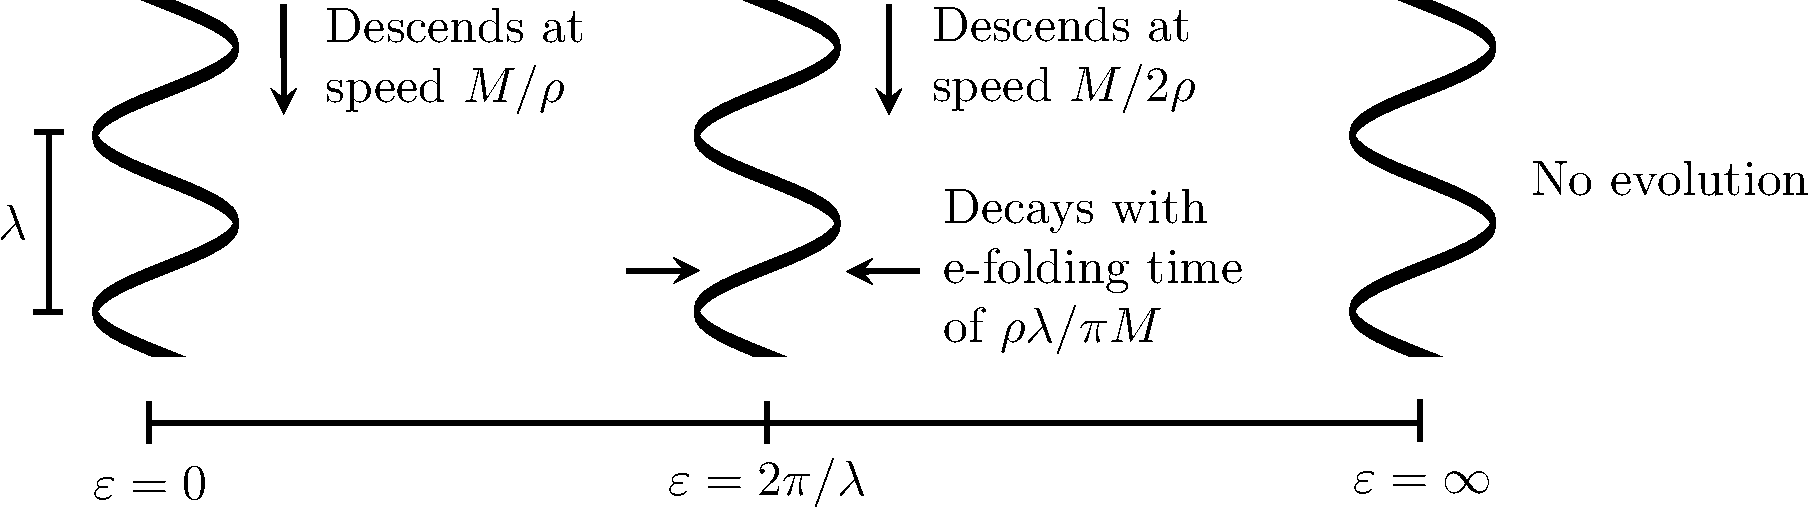
\includegraphics[width=6in]{../figures/17leshouches_sine.pdf}
\caption{The response of a sinusoidal tracer profile to moist convection with $\delta = \varepsilon$ and three values of $\varepsilon$: zero, the vertical wavenumber of the sinusoid, and infinity.}
\label{17leshouches_sine}
\end{center}
\end{figure}


\section{Free-tropospheric RH}


The previous section has given us a feel for the transient evolution of tracers in the moist-convecting atmosphere.  More relevant to climate, however, is the application of the bulk-plume equations to the steady-state profile of relative humidity.  Water vapor is the dominant greenhouse gas and the shortwave absorber, so it is critically important to understand the processes that set its distribution.


In the derivation that follows, we will let $q_v(z)$ represent the water-vapor mass fraction in the environment.  Since the environment occupies 99-99.9\% of the horizontal area at each height, $q_v(z)$ is also an excellent approximation for the specific humidity averaged over the entire area (both convection and environment) at height $z$.  Therefore, we will interchangeably refer to $q_v$ as the specific humidity of the environment and of the entire atmosphere.


For the convective plume, we will make two simplifying approximations.  First, we will assume that the convective plume carries no condensates.  This may sound a bit silly (after all, clouds are only visible because of their condensates), but the ratio of the condensate mass fraction to the water-vapor mass fraction is quite small within moist convection in the lower troposphere.  And, although we do not allow the convective plume to loft condensates, we still allow the convecting plume to condense water vapor; we just imagine that the resulting condensates are removed from the convective plume quickly, with some fraction rapidly falling to the surface and the remainder rapidly evaporating into the environment.  Second, we approximate the temperature of the two plumes to be equal at each height.  This ``zero-buoyancy plume approximation'' was introduced by \citet{singh2013}.  This may also sound a bit silly (after all, clouds only rise because they have some positive buoyancy), but that buoyancy is of only secondary importance to the atmosphere's water budget.  Furthermore, the typical buoyancy of tropical moist convection is only about 0.3 K \citep{13stereo}, which is quite small, indeed.  With these two approximations, the convective plume's mass fraction of total water (vapor plus condensates) is simply equal to the environment's saturation humidity, $q_v^*(z)$.


To begin, we must construct the bulk-plume equations for water vapor in an atmosphere with no net ascent or descent.  Let $M$ denote the convective mass flux (units of kg m$^{-2}$ s$^{-1}$), $e$ and $d$ denote the entrainment and detrainment rates (units of kg m$^{-3}$ s$^{-1}$), $c$ denote the condensation rate (units of kg m$^{-3}$ s$^{-1}$), and $\alpha$ the fraction of condensates formed at height $z$ that evaporate into the environment at height $z$.  We can then write down the following equations for the steady-state convective mass flux $M$, the humidity within clouds $q_v^*$, and the humidity within the environment $q_v$:
\begin{eqnarray}
\ppz M &=& e - d \label{M_bulk} \\
\ppz (M q_v^*) &=& e q_v - d q_v^* - c \label{qvs_bulk_1} \\
\ppz (-M q_v) &=& d q_v^* - e q_v + \alpha c \, . \label{qv_bulk_1}
\end{eqnarray}
Since $M$ is the total mass flux and $q_v$ is a mass fraction (as opposed to a mixing ratio), there should technically be a $-c$ on the right-hand side of equation (\ref{M_bulk}) to account for the loss of mass due to condensation.  For small $q_v^*$, as in Earth's atmosphere, this term has a negligible impact and its inclusion greatly complicates the equations, so it has been omitted\footnote{This choice is analogous to the treatment of mass in the Boussinesq equations, in which density is held constant for the purposes of the conservation-of-mass equation even though it is effectively removed and added by the ``heating'' $Q$ in the equation for buoyancy}.   Defining the fractional entrainment and detrainment rates as $\varepsilon = e/M$ and $\delta = d/M$, the mass flux $M$ can be eliminated from these equations to yield
\begin{eqnarray}
\ppz q_v^* &=& \varepsilon (q_v - q_v^*) - c/M \label{qvs_bulk_2} \\
- \ppz q_v &=& \delta (q_v^* - q_v) + \alpha c / M \, . \label{qv_bulk_2} 
\end{eqnarray}
The gross condensational heating is $Lc$ and the gross evaporative cooling is $\alpha Lc$.  Therefore, the precipitation efficiency PE is equal to $(Lc-\alpha Lc)/(Lc) = 1-\alpha$.


Writing $q_v$ as $q_v = \text{RH} q_v^*$ and assuming that the fractional variations in RH are small over the distance $1/\gamma$, i.e., $\ppz \log(\text{RH}) \ll \ppz \log(q_v^*)$, we can approximate these equations as
\begin{eqnarray}
-\gamma q_v^* &=& \varepsilon (\text{RH} - 1) q_v^* - c/M \label{bpc_2} \\
\text{RH} \gamma q_v^* &=& \delta (1 - \text{RH}) q_v^* + \alpha c/M \, . \label{bpe_2} 
\end{eqnarray}
These two equations can be solved for RH and $c/M$, giving
\begin{eqnarray}
\text{RH} &=& \frac{\delta + \alpha \gamma - \alpha \varepsilon}{\delta + \gamma - \alpha \varepsilon} \label{rh} \\
\frac{c}{M} &=& \frac{\delta + \gamma - \varepsilon}{\delta + \gamma - \alpha \varepsilon} \gamma q_v^* \, . \label{cond}
\end{eqnarray}
This derivation of equation (\ref{rh}) is replicated from \citet{13lapse}.


This expression for RH is particularly easy to understand if $\alpha=0$.  In that case, equation (\ref{rh}) simplifies to
\begin{equation}
\text{RH} \; = \; \frac{\delta}{\delta + \gamma} \, . \label{rh_ito_gamma_delta}
\end{equation}
Note that $1/\delta$ is the lengthscale over which convection moistens the environment towards saturation (by detraining saturated air into the clear air as it subsides), and $1/\gamma$ is the lengthscale over which subsidence drives RH towards zero (by adiabatic compression of the subsiding air, which drives up $q_v^*$).  The relative humidity is set by the balance between these two processes.  If $\delta$ is large, then the moistening effect of convection wins out over subsidence-driven drying, and RH is close to unity.  If $\delta$ is small, then the subsidence-driven ``drying'' dominates\footnote{The word ``drying'' is in quotation marks here because the adiabatic subsidence of a parcel does not change its $q_v$; it only increases is $q_v^*$, thereby leading to a decrease in RH.  Therefore, it is only a drying from the perspective of {\it relative} humidity.}, and RH is close to zero.


In the free troposphere, the relative humidity profile tends to have maximum values in the lower and upper troposphere, and a minimum in the middle troposphere.  We are now in a position to understand this characteristic ``C'' shape of the RH profile.  In the lower troposphere, $\gamma$ is small because the moist-adiabatic temperature lapse rate is small.  In the upper troposphere, $\delta$ is large because the mass flux is decreasing with height towards zero.  In both places, the RH is closer to one than zero.  In the middle troposphere, both $\delta$ and $\gamma$ are moderate and, in fact, tend to be of comparable magnitude.  That drives RH to values closer to a half.


Equation (\ref{rh}) also allows us to see how biases in a convective parameterization will affect free-tropospheric RH in a GCM.  A convective parameterization that has too little entrainment will also have too little detrainment (since the mass flux $M$ and, therefore, $\ppz M$ are largely constrained by clear-sky radiative cooling, and $\ppz M = e - d$), and this will tend to give a free troposphere that is too dry.  And, not surprisingly, a convective parameterization that has too high a precipitation efficiency (i.e., too low an $\alpha$) will also produce a free troposphere that is too dry.


The precipitation efficiency is notoriously difficult to quantify in observations.  For an atmosphere with no net ascent, however, we can place a bound on the precipitation efficiency simply by measuring RH.  Solving (\ref{rh}) for $\alpha$, we get
\begin{equation}
\alpha \; = \; \rh \frac{A}{B} \, , \label{alpha_rh_A_B}
\end{equation}
where
\begin{eqnarray}
A &=& \gamma - (1-\rh) \frac{\delta}{\rh} \label{a_num} \\
B &=& \gamma - (1-\rh) \;\; \varepsilon \, . \label{b_den}
\end{eqnarray}
Since $\alpha$ and RH are positive by definition, either $A$ and $B$ are both positive or both negative.  To determine their sign, consider $B$.  By equation (\ref{cond}), $B$ is equal to the gross condensation rate $c$ divided by the mass flux $M$ and $q_v^*$, all of which are positive.  Therefore, $A$ and $B$ are both positive.  Since $\delta$ is generally bigger than $\varepsilon$, $\delta/\rh$ is almost certainly bigger than $\varepsilon$, so $0 < A < B$.  Therefore, $A/B < 1$ and so $\alpha < \rh$.  Since $\pe = 1-\alpha$, this implies that $\pe > 1-\rh$.  In other words, an observation of RH automatically provides a lower bound on PE.  Figure \ref{17leshouches_precipeff} plots PE and $1-\rh{}$ for a cloud-resolving simulation of RCE.  As expected, PE is bounded from below by $1-\rh{}$.


\begin{figure}
\begin{center}
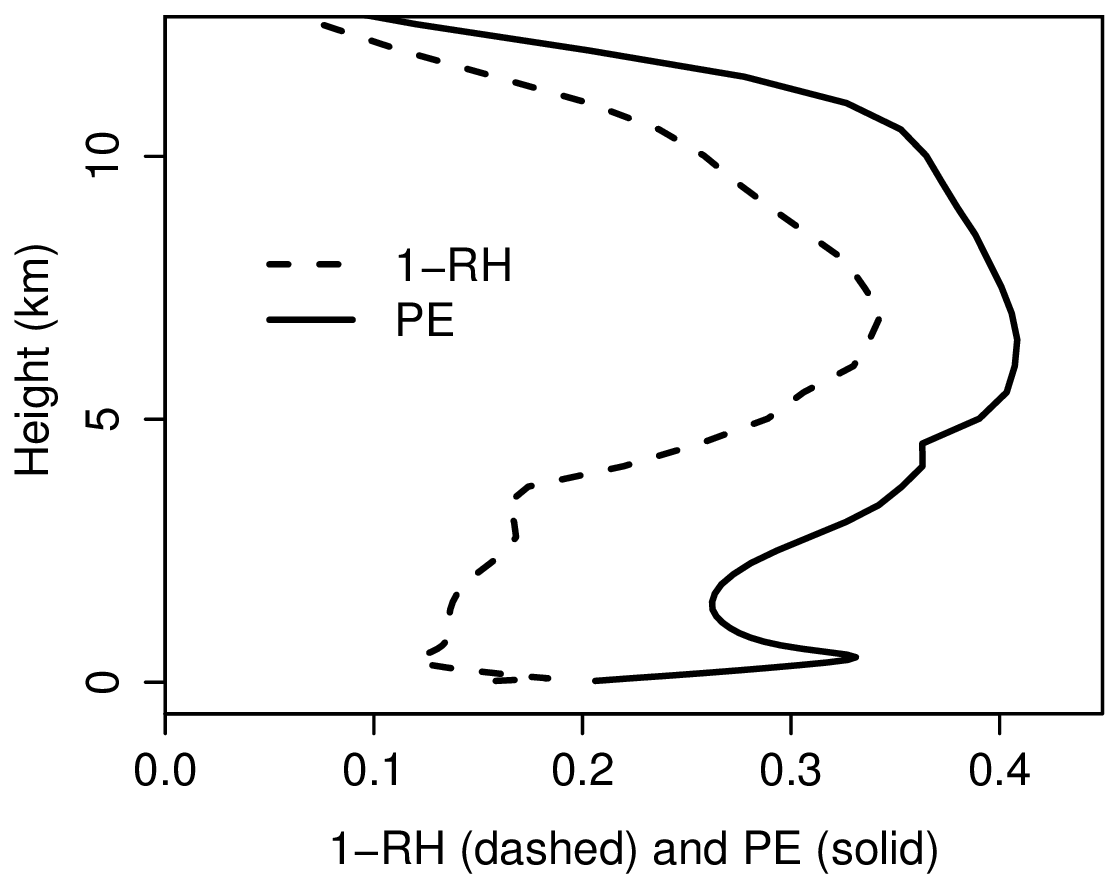
\includegraphics[width=4in]{../figures/17leshouches_precipeff.png}
\caption{(left) Profiles of (dashed) $1-\rh$ and (solid) precipitation efficiency for a cloud-resolving simulation of RCE.  Adapted from \citet{13lapse}.}
\label{17leshouches_precipeff}
\end{center}
\end{figure}


\section{Moist-entraining lapse rate}


In section \ref{sec_adiabatic_lapse}, we derived an expression for the moist-adiabatic lapse rate.  In reality, the lapse rate of the tropical free troposphere is larger than that for a moist adiabat; the real atmosphere is much closer to the temperature of entraining moist convection.  Following \citet{15cape}, we can derive an expression for the moist-entraining lapse rate by assuming that $M$, RH, and PE (i.e., $1-\alpha$) are all constant with height.  The constancy of $M$ with height then implies that $\varepsilon = \delta$, and the constancy of RH and $\alpha$ then implies that $\varepsilon$ and $\delta$ are both constant.


To set up the problem, we must write down two expressions for the vertical derivative of MSE$^*$ that can be combined to give an expression for $\Gamma$.  Using the zero-buoyancy plume approximation, MSE$^*$ of the environment is equal to MSE$^*$ of the convection.  Recalling the definitions $\mse^* = c_p T + L q_v^* + gz$ and $\gamma \equiv -\ppz \log(q_v^*)$, we can write 
\[
\ppz \mse{}^* \; = \; -c_p \Gamma + g - L \gamma q_v^* \, .
\]
Using equation (\ref{gamma}) for $\gamma$, we can write this as
\begin{equation}
\ppz \mse{}^* \; = \; g \left( 1 + \frac{q_v^* L}{R T} \right) - \Gamma \left( c_p + \frac{q_v^* L^2}{R_v T^2} \right) \, . \label{dhsdz_1}
\end{equation}


The second equation for $\mse{}^*$ is obtained by writing down the bulk-plume equation for the updraft MSE,
\begin{eqnarray}
\ppz \mse{}^* &=& \varepsilon (\mse{} - \mse{}^*) \nonumber \\
&=& \varepsilon L (q_v - q_v^*) \nonumber \\
&=& \varepsilon (\text{RH} - 1) L q_v^* \, . \label{dhsdz_2}
\end{eqnarray}
The assumption of constant $M$, RH, and $\alpha$ implies that $\varepsilon$ is proportional to $\gamma$.  Let us define the constant $a$ as $a = (1-\alpha)\varepsilon / \gamma$.  The entrainment rate, detrainment rate, the relative humidity from equation (\ref{rh}), and the condensation rate from (\ref{cond}) can then be written as
\begin{eqnarray}
\varepsilon \; = \; \delta &=& \frac{a\gamma}{1-\alpha} \label{app_eps_a} \\
\text{RH} &=& \frac{\alpha + a}{1 + a} \label{app_rh_a} \\
\frac{c}{M} &=& \frac{\gamma q_v^*}{1 + a} \, . \label{app_cond_a}
\end{eqnarray}
Substituting (\ref{app_eps_a}) and (\ref{app_rh_a}) into (\ref{dhsdz_2}), we get
\begin{equation}
\ppz \mse{}^* \; = \; - \frac{a}{a + 1} \gamma L q_v^* \, . \label{dhsdz_2_a}
\end{equation}
Note that $\gamma L q_v^* = -L\ppz q_v^*$, so this can be written as $\ppz \text{EMSE}^* = 0$, where
\begin{equation}
\text{EMSE}^* \; = \; c_p T + gz + \frac{Lq_v^*}{1+a} \label{app_emse}
\end{equation}
is a conserved variable for entraining parcels in the zero-buoyancy plume approximation much like MSE$^*$ is conserved for adiabatic parcels; we call this the entraining moist static energy (EMSE).


Finally, equating the right-hand sides of (\ref{dhsdz_1}) and (\ref{dhsdz_2_a}) and using (\ref{gamma}) to express $\gamma$ in terms of $\Gamma$, we can solve for $\Gamma$ to find
\begin{equation}
\Gamma \; = \; \frac{\displaystyle (1+a) g + \frac{q_v^* L g}{RT}}{\displaystyle (1+a)c_p + \frac{q_v^* L^2}{R_v T^2}} \, . \label{Gamma_a}
\end{equation}
If the entrainment rate is zero (i.e., $a=0$), then the moist-entraining lapse rate reduces to the moist-adiabatic lapse rate given in equation (\ref{moist_adiabatic_lapse}).


More interesting is the limit of infinite entrainment (i.e., $a \rightarrow \infty$), in which case the moist-entraining lapse rate reduces to the dry-adiabatic lapse rate $g/c_p$.  This is consistent with equation (\ref{app_cond_a}), which tells us that the condensation rate goes to zero.  At the same time, however, equation (\ref{app_rh_a}) tells us that the atmosphere becomes saturated.  We can understand all of this as follows.  An increase in the entrainment of subsaturated environmental air reduces the condensation rate and, therefore, steepens the lapse rate, pushing it towards the dry adiabat.  Meanwhile, an increase in entrainment implies an increase in detrainment, which moistens the environment, pushing it towards saturation.  For a very large entrainment rate, the environment is nearly saturated, but the entrainment rate is large enough that the entrainment of the slightly subsaturated environmental air places the condensation rate at a value near zero.


\section{Analytical theory for CAPE}


In the previous section, we learned that EMSE$^*$, defined in equation (\ref{app_emse}), is constant in RCE when $M$, RH, and PE are constant.  We can use this fact to derive an analytical expression for CAPE following \citet{15cape}.  From the fact that saturated EMSE$^*$ is constant with height in the environment, we know that
\begin{equation}
c_p T + gz_e(T) + \frac{L q_v^*[p_e(T),T]}{1+a} = c_p T_{\text{cb}} + \frac{L q_{v,\text{cb}}^*}{1+a} \, , \label{ze}
\end{equation}
where $T_{\text{cb}}$ is the cloud-base air temperature, $q_{v,\text{cb}}^*$ is the cloud-base saturation water-vapor mass fraction, $z_e(T)$ is the height profile as a function of environmental temperature, and $p_e$ is the pressure profile as a function of environmental temperature.


CAPE is the vertical integral of the buoyancy of a parcel as it is lifted {\it adiabatically} through the atmosphere.  The temperature of this adiabatically lifted parcel is governed by the MSE equation, given in equation (\ref{gov_mse}).  There, we see that the MSE of the parcel decreases with height in proportion to its buoyancy.  To good approximation, we can neglect that change in MSE so long as the characteristic height over which its buoyancy is expressed (which is typically about 10 km) is small compared to the scale height $c_p T/g$ (which is about 20-30 km, depending on the characteristic temperature)\footnote{To see why, imagine that we calculate the buoyancy of the adiabatically lifted parcel using conservation of MSE (i.e., neglecting the adiabatic decrease in MSE) and obtain from this a characteristic temperature anomaly (difference in temperature between a parcel and its surroundings) of $\Delta T$.  If we had properly accounted for the decrease in MSE, then the correction to the parcel's MSE would be
\[
\delta \mse{} \sim -\text{CAPE} \, .
\]
In the upper troposphere, where $q_v^*$ is small, this must be expressed as a change in temperature or, equivalently, a correction to $\Delta T$ on the order of
\[
\delta \Delta T \approx -\text{CAPE}/c_p \, .
\]
Defining $H$ as the characteristic height over which $\Delta T$ is expressed, then the correction to the CAPE will be on the order of
\begin{align}
\delta \text{CAPE} &\sim H \delta b \\
&= H g \frac{\delta \Delta T}{T} \\
&\approx -\frac{H g}{c_p T} \text{CAPE} \, ,
\end{align}
and this is small if $H \ll c_p T /g$, i.e., if the height over which the buoyancy is expressed is small compared to the scale height $c_pT/g \approx 30$ km.  In the current tropics, CAPE tends to be dominated by high buoyancy in the upper troposphere, the depth of which is small compared to 30 km.  Therefore, for a first-order approximation of CAPE, it is appropriate to calculate adiabatic-parcel ascent using strict conservation of MSE.}  Therefore, we will use strict conservation of MSE to approximate the properties of the adiabatic parcel.


For the adiabatic or ``undiluted'' parcel, we then know that
\begin{equation}
c_p T + gz_u(T) + L q_v^*[p_u(T),T] = c_p T_s + L q_{v,\text{cb}}^* \, , \label{zu}
\end{equation}
where $z_u(T)$ and $p_u(T)$ are the profiles of height and pressure, respectively, as functions of undiluted-parcel temperature.  If we subtract (\ref{ze}) from (\ref{zu}), we get
\[
g\left[ z_u(T) - z_e(T) \right] + L q_v^*[p_u(T),T] - \frac{L q_v^*[p_e(T),T]}{1+a} = \frac{a}{1+a} L q_{v,\text{cb}}^* \, .
\]
Thanks to the fact that $L q_v^*/R T \ll 1$ through most of the troposphere\footnote{The values of $q_v^*[p_u(T),T]$ and $q_v^*[p_e(T),T]$ are related to each other by
\begin{align*}
q_v^*[p_u(T),T] &= \frac{R p_v^*(T)}{R_v p_u(T)} \\
&\approx \frac{R p_v^*(T)}{R_v \left\{ p_e(T) - [z_u(T)-z_e(T)] \rho_e g \right\}} \\
&\approx \frac{R p_v^*(T)}{R_v p_e(T) \left\{ 1 - [z_u(T)-z_e(T)] g / RT \right\}} \\
&\approx \frac{R p_v^*(T)}{R_v p_e(T)} \left\{ 1 + [z_u(T)-z_e(T)] g / RT \right\} \\
&\approx q_v^*[p_e(T),T] \left\{ 1 + [z_u(T)-z_e(T)] g / RT \right\} \, .
\end{align*}
Using this more accurate expression for $q_v^*[p_u(T),T]$, we get
\[
\Delta z = \frac{a}{1+a} \frac{L}{g \left( 1 + \frac{L q_v^*}{R T} \right)} \left( q_{v,\text{cb}}^* - q_v^* \right) \, .
\]
By comparison to (\ref{delta_z}), we see that accounting for the difference between $q_v^*[p_u(T),T]$ and $q_v^*[p_e(T),T]$ modifies $\Delta z$ by a factor of $1 + L q_v^*/RT$.  At 300 K, $L q_v^*/RT$ is about $1/2$, and it decays exponentially as temperature decreases.  Therefore, over the vast majority of the troposphere for cloud-base temperatures below about 310 K, we can ignore this factor.}, $q_v^*[p_u(T),T]$ can be approximated as $q_v^*[p_e(T),T]$.  Therefore, this simplifies to
\begin{equation}
\Delta z(T) \approx \frac{a}{1+a} \frac{L}{g} \left( q_{v,\text{cb}}^* - q_v^* \right) \, , \label{delta_z}
\end{equation}
where $\Delta z(T) \equiv z_u(T) - z_e(T)$.  Figure \ref{17leshouches_profiles} shows plots of $z_e$ and $z_u$ for three different cloud-base temperatures and $a=0.2$.


\begin{figure}
\begin{center}
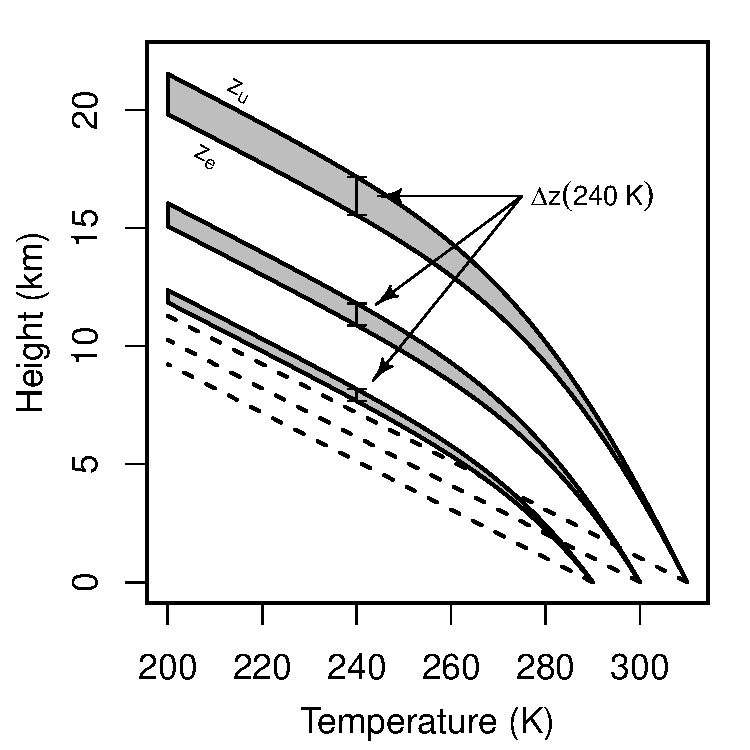
\includegraphics[width=4in]{../figures/17leshouches_profiles.pdf}
\caption{For $a=0.2$ and surface temperatures (really, cloud-base temperatures) of $T_s = 290$, 300, and 310 K, profiles of (solid) environmental and non-entraining-parcel temperature profiles calculated using the analytical expression in equation (11) of \citet{15cape} and (dashed) dry adiabats.  Note that CAPE is proportional to the shaded area between the two temperature profiles.}
\label{17leshouches_profiles}
\end{center}
\end{figure}


To get CAPE, we need the area between the two temperature curves plotted on $z$ and $T$ axes.  This is usually expressed as
\begin{equation}
\cape \approx \frac{g}{T_0} \int_{\text{cloud base}}^{\text{tropopause}} dz \, \Delta T(z) \, , \label{cape_dT}
\end{equation}
where $T_0$ is a characteristic tropospheric temperature (e.g., the average of the surface and tropopause temperatures), the tropopause is the assumed level of neutral buoyancy for the undiluted plume, and $\Delta T(z)$ is the temperature difference between the undiluted plume and the environment at height $z$.  But, another way to write this is
\begin{equation}
\cape \approx \frac{g}{T_0} \int_{T_{\text{tropopause}}}^{T_{\text{cloud base}}} dT \, \Delta z(T) \, . \label{cape_dz}
\end{equation}
The integrals in (\ref{cape_dT}) and (\ref{cape_dz}) are identical.  For our purposes, though, it is much more convenient to evaluate the integral in equation (\ref{cape_dz}).  Plugging in our expression for $\Delta z$, this becomes
\[
\cape \approx \frac{g}{T_0} \int_{T_{\text{tropopause}}}^{T_{\text{cloud base}}} dT \, \frac{a}{1+a} \frac{L}{g} \left( q_{v,\text{cb}}^* - q_v^* \right) \, .
\]
Over most of the temperature range of the troposphere, $q_v^* \ll q_{v,\text{cb}}^*$, so we can further approximate this as
\[
\cape \approx \frac{g}{T_0} \int_{T_{\text{tropopause}}}^{T_{\text{cloud base}}} dT \, \frac{a}{1+a} \frac{L}{g} q_{v,\text{cb}}^* \, .
\]
At this point, nothing in side the integral depends on $T$, so this integrates trivially to give
\begin{equation}
\cape \approx \frac{a}{1+a} L q_{v,\text{cloud base}}^* \frac{T_{\text{cloud base}} - T_{\text{tropopause}}}{T_0} \, . \label{cape_simple}
\end{equation}
As expected, CAPE increases with the entrainment rate, i.e., with $a$.  Most importantly, we see that CAPE increases in proportion to $q_v^*$ at the cloud base; this means that CAPE experiences Clausius-Clapeyron scaling, increasing exponentially with surface temperature, which is closely tied to the cloud-base temperature.  This dependence of CAPE on surface temperature is illustrated in Figure \ref{17leshouches_cape}; note the log axis.  This exponential dependence on surface temperature has implications for the intensity of storms since CAPE is the reservoir of energy that storms can tap to generate damaging winds, hail, and lightning.


\begin{figure}
\begin{center}
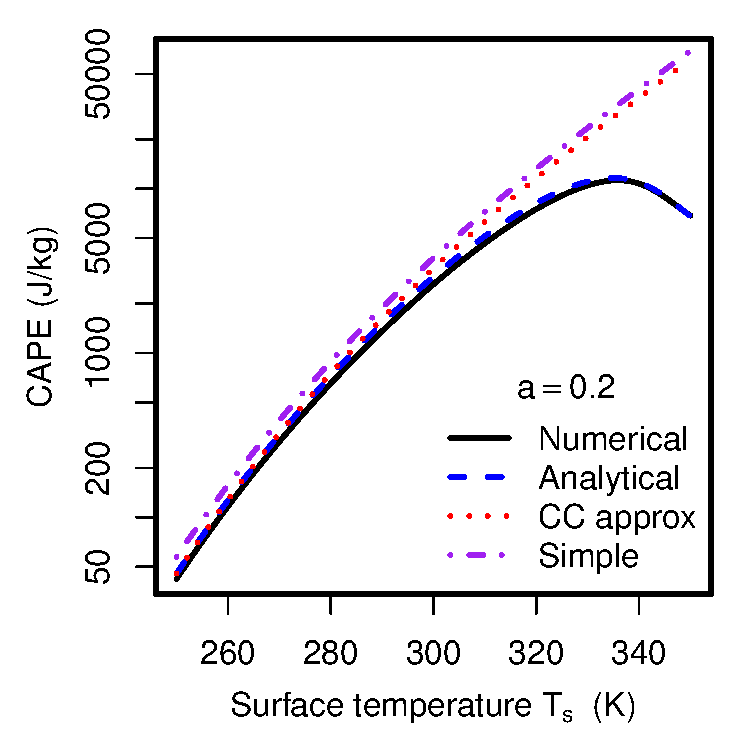
\includegraphics[width=4in]{../figures/17leshouches_cape.pdf}
\caption{CAPE as a function of surface temperature $T_s$ (really, cloud-base temperature) for $a=0.2$ as calculated using (black solid) numerical integration, (blue dashed) the analytical expression for CAPE given by equation (12) of \citet{15cape}, and (red dotted) the approximate analytical expression for CAPE in equation (17) of \citet{15cape}, which exhibits CC scaling.  Also plotted is the simple approximation for CAPE given here in equation (\ref{cape_simple}).  Adapted from Figure 5 of \citet{15cape}.}
\label{17leshouches_cape}
\end{center}
\end{figure}




\clearpage
\bibliography{17leshouches_notes}

\end{document}






\section{Moist equations}


That is dry.  If we add water, we need to keep track of at least two types: vapor and liquid.  Vapor can condense into liquid, liquid can evaporate into vapor, and liquid can fall relative to the air, causing water to fall into or out of the box even if the air is not moving.  Denoting the condensation rate by $c$, which will also represent evaporation by being negative, we can write
\begin{align}
\ppt (\rho q_v) + \grad \cdot (\rho q_v \vec{u}) &= -c \\
\ppt (\rho q_l) + \grad \cdot \left[ \rho q_l (\vec{u} - V_t \hat{z}) \right] &= c \, .
\end{align}
We can write the free-fall fluxes as an effective source as
\[
\ppt (\rho q_l) + \grad \cdot \left[ \rho q_l (\vec{u} + \vec{V}_t) \right] = c + \ppz \cdot (\rho q_l V_t) \, .
\]
Next, we must recognize that, since our $\rho$ is the total air mass (not just the dry air mass), we must account for the loss of mass due to free fall in the $\rho$ equation.  Therefore, we get
\begin{align}
\ppt \rho + \grad \cdot (\rho \vec{u}) &= \ppz \cdot (\rho q_l V_t) + S_{\text{vapor @ surface}} \\
\ppt (\rho \vec{u}) + \grad \cdot (\rho \vec{u} \vec{u}) &= \vec{g} - \grad p + \vec{S}_{\text{momentum @ surface}} \\
\ppt (\rho E) + \grad \cdot (\rho E \vec{u}) &= Q - \grad \cdot (p \vec{u}) + S_{\text{energy @ surface}} \label{gov_energy_moist} \\
\ppt (\rho q_v) + \grad \cdot (\rho q_v \vec{u}) &= -c + S_{\text{vapor @ surface}} \label{gov_qv_moist} \\
\ppt (\rho q_l) + \grad \cdot \left[ \rho q_l (\vec{u} + \vec{V}_t) \right] &= c + \ppz \cdot (\rho q_l V_t) \\
p &= R\rho T \, .
\end{align}
Here, $E = c_vT + q_vE_{0v}$.  We have also added the equation of state for $p$.  That is all the dynamics that we need to build a climate model.  (Coriolis forces and curvature terms are all caused by choosing a bad reference frame, e.g., an east, north, and up frame that rotates with the planet.)  We only need to add some physics: pick a radiative transfer scheme for $Q$, and pick a microphysics scheme for $c$ and $V_t$.


Since water vapor is a small-mixing-ratio trace gas, we can approximate this in the free troposphere (away from the surface) by
\begin{align}
\ppt \rho + \grad \cdot (\rho \vec{u}) &= 0 \\
\ppt (\rho \vec{u}) + \grad \cdot (\rho \vec{u} \vec{u}) &= \vec{g} - \grad p \\
\ppt (\rho E) + \grad \cdot (\rho E \vec{u}) &= Q - \grad \cdot (p \vec{u}) \\
\ppt (\rho q_v) + \grad \cdot (\rho q_v \vec{u}) &= -c \\
p &= R\rho T \, .
\end{align}

